%%%%%%%%%%%%%%%%%%%%%%%%%%%%%%%%%%%%%%%%%
% The Legrand Orange Book
% LaTeX Template
% Version 3.1 (February 18, 2022)
% Compiling this template:
% This template uses biber for its bibliography and makeindex for its index.
% When you first open the template, compile it from the command line with the 
% commands below to make sure your LaTeX distribution is configured correctly:
%
% 1) pdflatex mainv2
% 2) makeindex mainv2.idx -s indexstyle.ist
% 3) biber mainv2
% 4) pdflatex mainv2 x 2


%Atención
%Está prohibido usar simbolos en \index{•}
% After this, when you wish to update the bibliography/index use the appropriate
% command above and make sure to compile with pdflatex several times 
% afterwards to propagate your changes to the document.
%
%%%%%%%%%%%%%%%%%%%%%%%%%%%%%%%%%%%%%%%%%

%----------------------------------------------------------------------------------------
%	PACKAGES AND OTHER DOCUMENT CONFIGURATIONS
%----------------------------------------------------------------------------------------

\documentclass[
	12pt, % Default font size, select one of 10pt, 11pt or 12pt
	fleqn, % Left align equations
	a4paper, % Paper size, use either 'a4paper' for A4 size or 'letterpaper' for US letter size
	oneside, % Uncomment for oneside mode, this doesn't start new chapters and parts on odd pages (adding an empty page if required), this mode is more suitable if the book is to be read on a screen instead of printed
]{LegrandOrangeBook}

% Book information for PDF metadata, remove/comment this block if not required 
\hypersetup{
	pdftitle={Pasos por Telecomunicaciones II}, % Title field
	pdfauthor={Jose Hancco}, % Author field
	pdfsubject={Educación}, % Subject field
	pdfkeywords={Telecomunicaciones, UNSA, Pregrado, Señales}, % Keywords
	pdfcreator={LaTeX}, % Content creator field
}

\addbibresource{sample.bib} % Bibliography file

\definecolor{ocre}{RGB}{63, 76, 83} % Define the color used for highlighting throughout the book, replace it with average color for a better presentation:
% Background.pdf -> Average color=63,76,83
% Background1.pdf -> Average color=31,31,40
% Background2.pdf -> Average color=123,119,101
% Background3.pdf -> Average color=103,61,76
\chapterimage{Final1.jpg} % Chapter heading image
\chapterspaceabove{6.5cm} % Default whitespace from the top of the page to the chapter title on chapter pages
\chapterspacebelow{6.75cm} % Default amount of vertical whitespace from the top margin to the start of the text on chapter pages

%----------------------------------------------------------------------------------------

\begin{document}

%----------------------------------------------------------------------------------------
%	TITLE PAGE
%----------------------------------------------------------------------------------------

\begingroup
\thispagestyle{empty} % Suppress headers and footers on the title page
\begin{tikzpicture}[remember picture,overlay]
\node[inner sep=0pt] (background) at (current page.center) {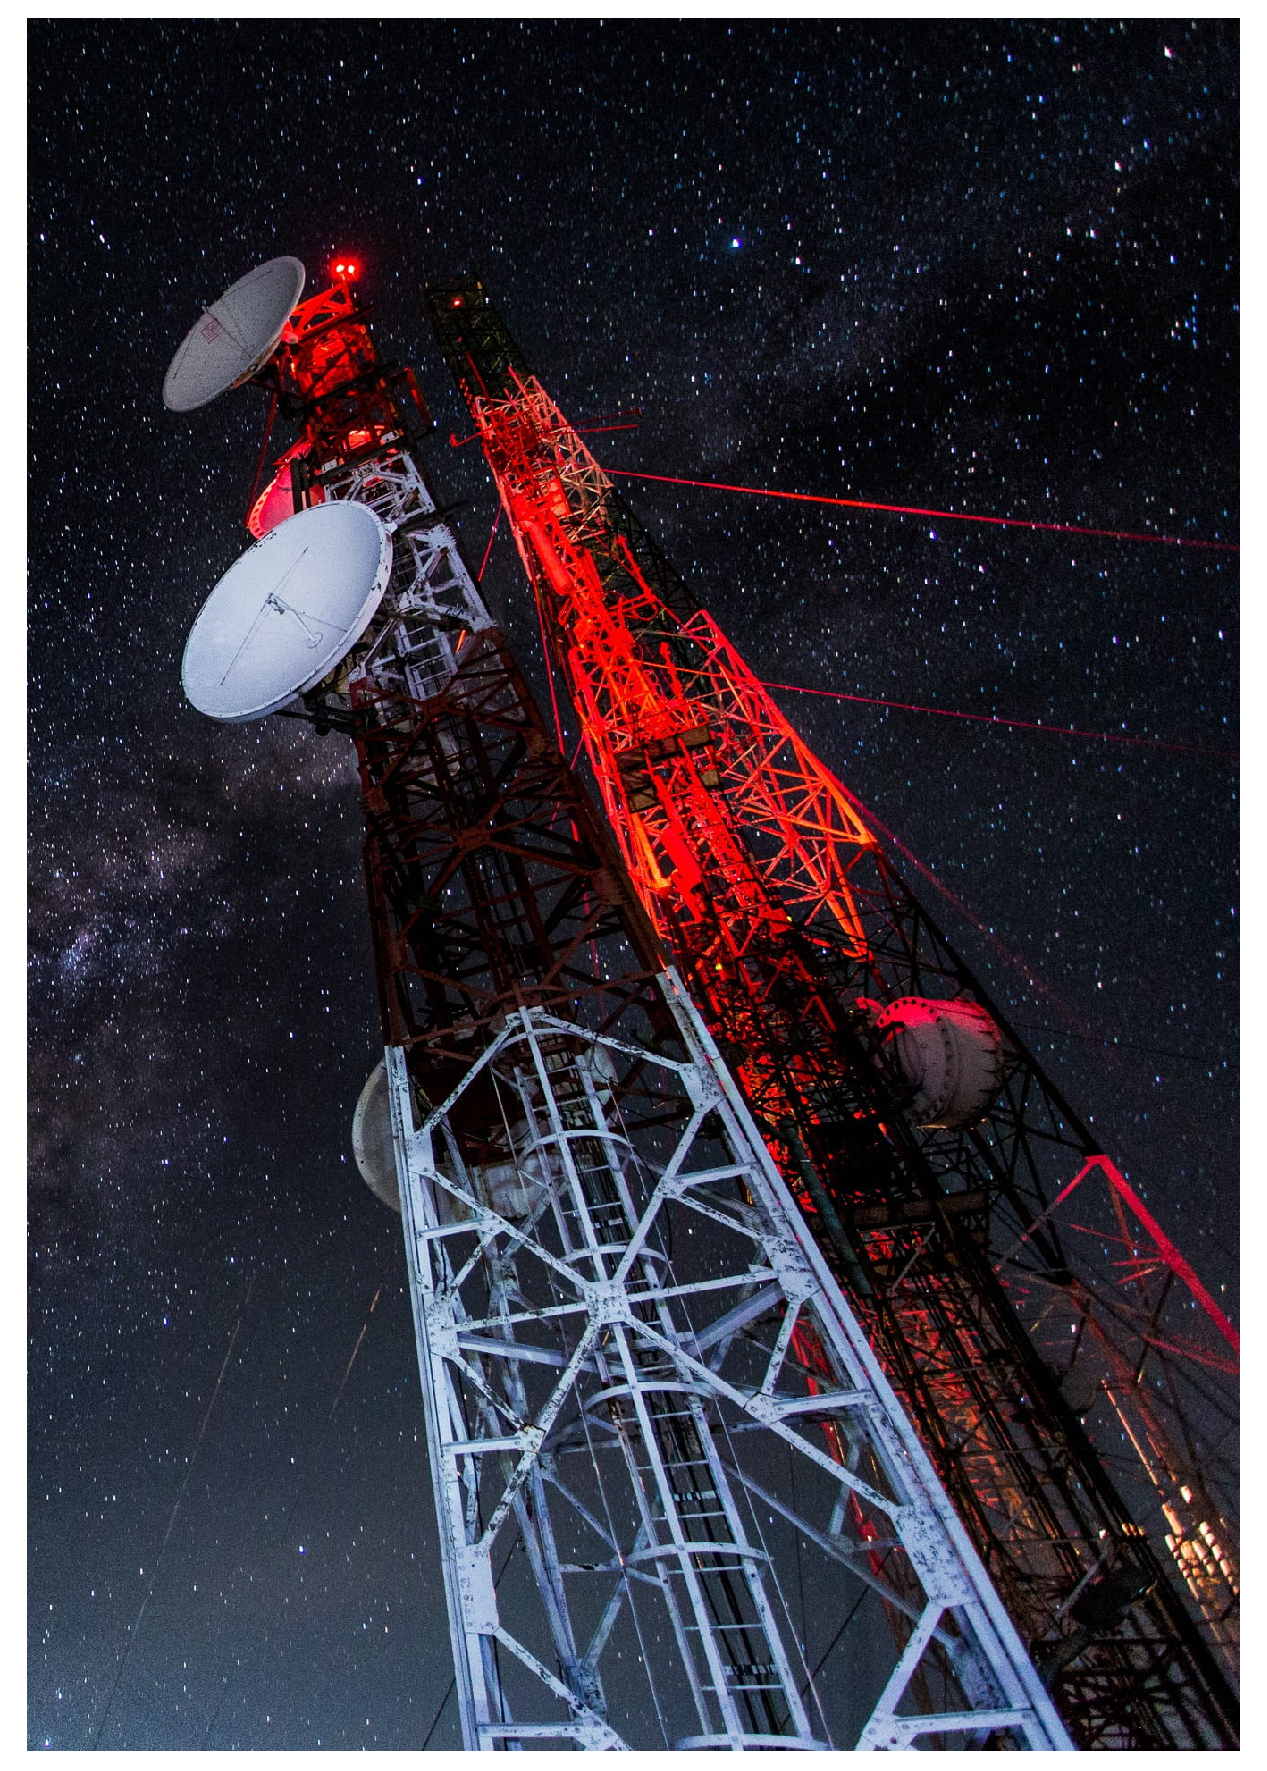
\includegraphics[width=\paperwidth]{background1.pdf}};%here you change your bookcover background
\draw (current page.center) node [fill=ocre!30!white,fill opacity=0.6,text opacity=1,inner sep=1cm]{\Huge\centering\bfseries\sffamily\parbox[c][][t]{\paperwidth}{\centering Pasos por Telecomunicaciones II\\[15pt] % Book title
{\Large Notas de un estudiante}\\[20pt] % Subtitle
{\huge Jose Antonio Hancco M.}}}; % Author name
\end{tikzpicture}
\vfill
\endgroup

%----------------------------------------------------------------------------------------
%	COPYRIGHT PAGE
%----------------------------------------------------------------------------------------

\newpage
~\vfill
\thispagestyle{empty}

\noindent Copyright \copyright\ 2022 Jose Hancco\\ % Copyright notice

\noindent \textsc{Libro libre de usos}\\ % Publisher

\noindent \textsc{https://github.com/Yasperterian}\\ % URL

\noindent Con licencia de Creative Commons Attribution-NonCommercial 3.0 Unported License (la ``Licencia''). No puede usar este archivo excepto de conformidad con la Licencia. Puede obtener una copia de la Licencia en \url{http://creativecommons.org/licenses/by-nc/3.0}. A menos que lo exija la ley aplicable o se acuerde por escrito, el software distribuido bajo la Licencia se distribuye \textsc{``tal cual'', sin garantías ni condiciones de ningún tipo}, ya sea expresa o implícita. Consulte la Licencia para conocer el idioma específico que rige los permisos y las limitaciones en virtud de la Licencia.\\ % License information, replace this with your own license (if any)

\noindent \textit{Primera edición, septiembre 2022} % Printing/edition date

\noindent Si existe algún error, crees que una sección se puede mejorar o dar cualquier tipo de \textit{feedback} acerca del libro no dudes y mándame un correo a \textit{jhanccoma@unsa.edu.pe}, te responderé lo más pronto que pueda y gracias por mejorar este libro de todos y para todos.
%----------------------------------------------------------------------------------------
%Dedicate
%----------------------------------------------------------------------------------------
\clearpage
\begin{center}
    \thispagestyle{empty}
    \vspace*{\fill}
    \textit{Realmente no sé a quien dedicar este texto, pues no es más que una recopilación de lo que voy aprendiendo para convertirme en ingeniero en telecomunicaciones, visto de manera dedico este libro a todos los estudiantes que por lo menos toman en cuenta la información contenida en el libro y más aún con las ganas de aprender de otro estudiante, como lo soy yo.}
    \vspace*{\fill}
\end{center}
\clearpage
%----------------------------------------------------------------------------------------
%	TABLE OF CONTENTS
%----------------------------------------------------------------------------------------

%\usechapterimagefalse % If you don't want to include a chapter image, use this to toggle images off - it can be enabled later with \usechapterimagetrue

\chapterimage{chapter_head_generalindex3.pdf} % Table of contents heading image

\pagestyle{empty} % Disable headers and footers for the following pages

\tableofcontents % Print the table of contents itself

\cleardoublepage % Forces the first chapter to start on an odd page so it's on the right side of the book

\pagestyle{fancy} % Enable headers and footers again
%----------------------------------------------------------------------------------------
%	PART
%----------------------------------------------------------------------------------------
\section*{Libros recomendados:}
\begin{itemize}
\item Fundamentos de circuitos eléctricos\cite{alexander2013fundamentos}
\item Signals and Systems Using MATLAB\cite{chaparro2018signals}
\item Procesamiento de señales analógicas y digitales\cite{ambardar1995analog}
\item Física Para Ciencias E Ingeniería. Vol 1\cite{serway2018fisica1}
\item Física Para Ciencias E Ingeniería. Vol 2\cite{serway2018fisica2}
\item Cálculo de una variable: trascendentes tempranas. 7ma edición \cite{stewart12calculo}
\item Análisis de Fourier\cite{hsu1998analisis}
\item Matemáticas Avanzadas Para Ingeniería\cite{o2014matematicas}
\item Métodos numéricos para ingenieros\cite{chapra2013metodos}
\item Comunicaciones y redes de computadores\cite{stallings2004comunicaciones}
\item Electrónica: teoría de circuitos y dispositivos electrónicos\cite{boylestad1989electronica}
\item Fundamentos de sistemas digitales\cite{floyd2006fundamentos}
\item Tratamiento de señales en tiempo discreto\cite{oppenheim2011tratamiento}
\item Tratamiento digital de señales\cite{proakis2007tratamiento}
\item Sistemas de comunicación digitales y análogos\cite{couchsistemas}
\item Data communication and networking\cite{forouzan2007data}
\item Life Pre-Intermediate 2e\cite{hughes2017life}
\item Redes de computadoras\cite{tanenbaum2012computer}
\item Líneas de transmisión\cite{velalineas1999}
\end{itemize}
%----------------------------------------------------------------------------------------
%	NEW CHAPTER
%----------------------------------------------------------------------------------------
\part{Antenas}
\chapterimage{chapter_head_ANT.pdf} % Chapter heading image

\chapter{Unidad I}
\section{Introducción}
Como siempre, antes de este curso hay que recordar algunos términos o conceptos para poder entender cosas que se vienen. Empezamos con las unidades logarítmicas:
\begin{align*}
Belio&=\log\left(\frac{P_{out}}{P_{in}}\right)\\
Decibelio(dB)&=10\cdot\log\left(\frac{P_{out}}{P_{in}}\right)\\
Decibelio(dB)&=20\cdot\log\left(\frac{V_{out}}{V_{in}}\right)\\
Neper(Np)&=ln\left(\frac{V_{out}}{V_{in}}\right)
\end{align*}
Asimismo debemos tener en cuenta las demás medidads respecto a un valor como 1mW, 1W, 1V, etc.\footnote{Estas puedes ser vistas en la sección \textbf{Decibelios} en el capítulo de \textbf{Ingeniería en mantenimiento}.}
Otros conceptos importantes a recordar son:
\begin{definition}[Longitud de Onda]
\begin{equation}
\lambda=\frac{v}{f}
\end{equation}
Donde:
\begin{itemize}
\item $\lambda$: Longitud de onda. (m)
\item \textbf{v}: Velocidad, si el medio es el aire o espacio libre: $v=c=3\times\basedec{8}$ m/s (m/s)
\item $f$: Frecuencia. (Hz)
\end{itemize}
\end{definition}
\begin{definition}[Temperatura]
\begin{equation}
\frac{°C}{5}=\frac{°F-32}{9}=\frac{K-273}{5}=\frac{R-492}{9}
\end{equation}
Despejando podemos obtener:
\begin{align*}
°C=\frac{5}{9}\left(°F-32\right)\\
K=°C+273\\
R=°F+460
\end{align*}
\end{definition}
Además debemos recordar las bandas y frecuencias designadas por la ITU:
\begin{table}[H]
\centering
\begin{tabular}{|c|c|c|c|}
\hline
\rowcolor[HTML]{9698ED} 
N° de banda & Rango de frecuencia & Indicativo & Propagación                    \\ \hline
2           & 30-300 Hz           & ELF        & Onda terrestre                 \\ \hline
3           & 0.3-3 KHz           & SLF        & Onda terrestre                 \\ \hline
4           & 3-30 KHz            & VLF        & Onda terrestre                 \\ \hline
5           & 30-300 KHz          & LF         & Onda terrestre y superficial   \\ \hline
6           & 0.3-3 MHz           & MF         & Onda superficial               \\ \hline
7           & 3-30 MHz            & HF         & Onda superficial y Ionosférica \\ \hline
8           & 30-300 MHz          & VHF        & Onda Ionosférica y directa     \\ \hline
9           & 0.3-3 GHz           & UHF        & Onda directa                   \\ \hline
10          & 3-30 GHz            & SHF        & Onda directa                   \\ \hline
11          & 30-300 GHz          & EHF        & Onda directa e infrarojo       \\ \hline
12          & 0.3-3 THz           &            & Luz infraroja                  \\ \hline
13          & 3-30 THz            &            & Luz infraroja                  \\ \hline
14          & 30-300 THz          &            & Luz infraroja                  \\ \hline
15          & 0.3-3 PHz           &            & Luz visible                    \\ \hline
16          & 3-30 PHz            &            & Luz ultravioleta               \\ \hline
17          & 30-300 PHz          &            & Rayos X                        \\ \hline
18          & 0.3-3 EHz           &            & Rayos X                        \\ \hline
19          & 3-30 EHz            &            & Rayos cósmicos                 \\ \hline
\end{tabular}
\caption{Designación de bandas CCIR por la ITU.}
\end{table}
Los medios de transmisión:
\begin{table}[H]
\resizebox{\textwidth}{!}{
\begin{tabular}{|c|c|c|c|}
\hline
\rowcolor[HTML]{9698ED} 
Medio de transmisión                                                                         & Banda de frecuencia & Longitud de onda & Aplicación principal                                                                                                                                         \\ \hline
\begin{tabular}[c]{@{}c@{}}Par de alambres,\\ cable multipar\end{tabular}                    & 30-300 Hz           & 10000-1000 Km    & Comunicación submarina                                                                                                                                       \\ \hline
\begin{tabular}[c]{@{}c@{}}Par de alambres,\\ cable multipar\end{tabular}                    & 0.3-3 KHz           & 1000-100 Km      & \begin{tabular}[c]{@{}c@{}}Telefonía, transmisión de datos,\\ telex, fax.\end{tabular}                                                                       \\ \hline
\begin{tabular}[c]{@{}c@{}}Par de alambres,\\ cable multipar,\\ ondas de tierra\end{tabular} & 3-30 KHz            & 100-10 Km        & \begin{tabular}[c]{@{}c@{}}Telefonía de onda portadora baja,\\ capacidad, navegación y radiotelegrafía.\end{tabular}                                         \\ \hline
\begin{tabular}[c]{@{}c@{}}Par de alambres,\\ ondas de tierra\end{tabular}                   & 30-300 KHz          & 10-1 Km          & \begin{tabular}[c]{@{}c@{}}Telefonía de onda portadora mediana\\ capacidad, radiofaro, navegación,\\ radiodifusión onda larga.\end{tabular}                  \\ \hline
\begin{tabular}[c]{@{}c@{}}Cable coaxial, ondas\\ de cielo\end{tabular}                      & 0.3-3 MHz           & 1000-100 m       & \begin{tabular}[c]{@{}c@{}}Radiodifusión, AM, radio aficionados,\\ radio móvil.\end{tabular}                                                                 \\ \hline
\begin{tabular}[c]{@{}c@{}}Cable coaxial, cable UTP cat 3-4,\\ ondas de cielo\end{tabular}   & 3-30 MHz            & 100-10m          & \begin{tabular}[c]{@{}c@{}}Radio aficionados, comunicaciones milirares,\\ marítimas, radio telefonía movil.\end{tabular}                                     \\ \hline
\begin{tabular}[c]{@{}c@{}}Cable coaxial, cable UTP cat 5,\\ ondas directas\end{tabular}     & 30-300 MHz          & 10-1 m           & \begin{tabular}[c]{@{}c@{}}TV, radiodifusión FM, multiacceso radial,\\ radio enlaces, direccionales.\end{tabular}                                            \\ \hline
Ondas directas                                                                               & 0.3-3 GHz           & 100-10 cm        & \begin{tabular}[c]{@{}c@{}}TV, telemetría por radar, comunicaiones\\ militares por satélite, telefonía celular, radio\\ de espectro ensanchado.\end{tabular} \\ \hline
Guía de onda, línea visual                                                                   & 3-30 GHz            & 10-1 cm          & \begin{tabular}[c]{@{}c@{}}Comunicaiones vía satélite, radio enlace\\ direccional analógico y digítal, operación\\ aérea por radar.\end{tabular}             \\ \hline
Guía de onda, línea visual.                                                                  & 30-300 GHz          & 1-0.1 cm         & \begin{tabular}[c]{@{}c@{}}Comunicación militar por satelite, \\ radio astronomia, aterrizaje por radar.\end{tabular}                                        \\ \hline
Fibra óptica                                                                                 & 100-1000 THz        & 3-0.3 pm         & \begin{tabular}[c]{@{}c@{}}Telefonia muy alta capacidad, servicios de\\ banda ancha (SONET, SDH y ATM),\\ video conferencia, CATV por F.O.\end{tabular}      \\ \hline
\end{tabular}
}
\end{table}
\subsection{Ancho de banda y capacidad de información}\index{Ancho de banda y capacidad de información}
Las limitaciones más importantes para el funcionamiento de una sistema de comunicaciones son el \textbf{ruido} y el \textbf{ancho de banda}. El ancho de banda de un canal de comunicación es la diferencia entre la frecuencia máxima y mínima que puede pasar por el canal. El ancho de banda de un canal de comunicación debe ser igual o mayor que el ancho de banda de la información.
\begin{definition}[Ley de Hartley]
Es la medida de cuanta información se puede transferir a través de un sistema de comunicaciones en un determinado tiempo.
\begin{equation}
I\approx B\times t
\label{eq:hartley}
\end{equation}
Donde:
\begin{itemize}
\item \textbf{I}: Capacidad de información.
\item \textbf{B}: Ancho de banda. (Hz)
\item \textbf{t}: Tiempo de transmisión. (s)
\end{itemize}
\end{definition}
\begin{notation}
Se requieren \textbf{3 KHz} de ancho de banda para transmitir las señales telefónicas con calidad de voz.\\
Se asigna \textbf{200 KHz} para transmisión comercial de FM para música, con alta fidelidad.\\
Se requieren casi \textbf{6 MHz} de ancho de banda para emitir señales de televisión de alta calidad
\end{notation}
Otra medida que debemos saber es:
\begin{definition}[Capacidad de información de un canal digital]
Shannon relacionó la capacidad de información de un canal de comunicaciones, en bits por segundo (bps), con el ancho de banda y la relación señal a ruido: 
\begin{equation}
I=B\cdot\log_2(1+S/N)
\label{eq:shannon}
\end{equation}
Donde:
\begin{itemize}
\item I: Capacidad de información. (bps)
\item B: Ancho de banda. (Hz)
\item S/N: Relación señal a ruido.
\end{itemize}
\end{definition}
\subsection{Ruido}\index{Ruido}
Energía eléctrica \textbf{no deseable} presente en la banda útil del circuito de comunicación. Se puede clasificar el ruido en dos categorías:
\begin{enumerate}
\item \textbf{Correlacionado}: Solo existe \textbf{cuando hay una señal}. Es aquel que se relaciona mutuamente con la señal, y no puede estar en un circuito a menos que haya una señal de entrada.
Se produce por amplificación no lineal, e incluye la distorsión armónica (cuando se producen las armónicas no deseadas de una señal, debido a una amplificación no lineal) y de intermodulación (generación de frecuencias indeseables de suma o diferencia), ya que las dos son formas de distorsión no lineal.
\item \textbf{No Correlacionado}: Está presente \textbf{siempre}, haya o no señal. El ruido no correlacionado puede sub dividirse en dos categorías generales:
\begin{enumerate}
\item \textbf{El Ruido Externo }es el que se genera fuera del dispositivo o circuito. Hay tres causas principales de ruido Externo:
\begin{enumerate}
\item \textbf{Ruido atmosférico}: Perturbaciones eléctricas naturales. Electricidad estática (rayos)
\item \textbf{Ruido extraterrestre}: Señales eléctricas originadas fuera de la atmósfera terrestre (solar y cósmico)
\item \textbf{Ruido hecho por el hombre}: Su puente principal son mecanismos que producen chispas, ruido industrial (conmutadores, generadores, lámparas fluorescentes)
\end{enumerate}
\item \textbf{El Ruido Interno} es la interferencia eléctrica generada dentro de un dispositivo o circuito. Las causas principales son:
\begin{enumerate}
\item \textbf{Ruido Térmico}: Asociado con el movimiento rápido y aleatorio de electrones libre, producido por la agitación térmica.
\item \textbf{Ruido de Tiempo de Tránsito}: Variación irregular y aleatoria, producida por la modificación de una corriente de portadores, cuando pasa de la entrada a la salida de un dispositivo.
\item \textbf{Ruido de Disparo}: Se debe a la llegada aleatoria de portadoras al elemento de salida de un dispositivo electrónico (diodo, FET, transistor bipolar).
\end{enumerate}
\end{enumerate}
\end{enumerate}
\subsection{Ruido térmico}\index{Ruido térmico}
Es el movimiento \textbf{aleatorio} de los electrones libres dentro de un conductor, causado por la agitación térmica. Lamentablemente, este ruido está a lo largo de todo el espectro electromagnético.
Llamado también: Movimiento Browniano por su descubridor Robert Brown, Ruido de Johnson en honor a quien lo relacionó con el movimiento de los electrones y Ruido Blanco porque se produce en todas las frecuencias.
\begin{definition}[Potencia de ruido térmico]
\begin{equation}
P_{tn}=K\cdot T\cdot B
\label{eq:ruido termico}
\end{equation}
Donde:
\begin{itemize}
\item $P_{tn}$: Potencia del ruido  térmico\footnote{tn:thermal noise o ruido térmico.} (W)
\item \textbf{K:} Constante de Boltzmann= $1.38\times\basedec{-23} J/°K$.
\item \textbf{T}: Temperatura absoluta. (°K)
\item \textbf{B}: Ancho de banda. (Hz)
\end{itemize}
Alternativamente, el ruido térmico puede ser expresado en dBm, para ello debemos usar la siguiente expresión comparada con un 1mW:
\begin{equation}
P_{tn}(dBm)=10\cdot\log\left(\frac{K\cdot T\cdot B}{0.001}\right)
\label{eq:ruido termico log}
\end{equation}
En temperatura ambiente (17 C o 290 K), el ruido térmico ambiente:
\begin{equation}
P_{tn}(dBm)=-174 dBm+10\log(B)
\label{eq:ruido termico ambiente}
\end{equation}
\end{definition}
\begin{definition}[Voltaje ruido térmico]
\begin{equation}
V_{tn}=\sqrt{4\cdot R\cdot K\cdot T\cdot B}
\label{eq:voltaje ruido termico}
\end{equation}
Donde:
\begin{itemize}
\item \textbf{R}: Resistencia interna. ($\Omega$)
\item \textbf{$V_{tn}$}: Voltaje RMS del ruido. (V)
\end{itemize}
\end{definition}
\begin{notation}
Para la máxima potencia transferencia de potencia $R_L=R_I$.
\end{notation}
\begin{definition}[Relación señal a ruido-SNR]
Es la relación en decibelios entre la potencia de la señal(S) y la potencia del ruido(N):
\begin{equation}
\label{eq:snr}
SNR=10\log_{10}\left(\frac{S}{N}\right)=20\log_{10}\left(\frac{V_s}{V_n}\right)
\end{equation}
\end{definition}
\begin{remark}
El \textbf{factor a ruido} se define como el cociente entre la potencia SNR de entrada y potencia SNR de salida. Por consecuencia, la \textbf{cifra de ruido} es el factor de ruido expresado en dB.
\end{remark}
\begin{notation}
Para voltaje, 6dB indica que la salida es dos veces el valor de la entrada, es decir: Si la entrada es 1, la salida será 2. Para potencia, 3dB indica lo mismo: el valor de la salida es dos veces el valor de la entrada.
\end{notation}
\subsection{Ángulo crítico}\index{Ángulo crítico}
Debemos recordar ecuaciones como Ley de Snell,
\begin{definition}[Ley de Snell]
\begin{align}
n_1\sin\theta_1&=n_2\sin\theta_2\\
\sqrt{\epsilon_1}\sin\theta_1&=\sqrt{\epsilon_2}\sin\theta_2
\label{eq:snell}
\end{align}
Donde:
\begin{itemize}
\item $n$: Indice de refracción.
\item $\theta$ Ángulo de refracción.
\item $\epsilon$: Permitividad relativa del material.
\end{itemize}
\end{definition}
\begin{figure}[H]
\centering
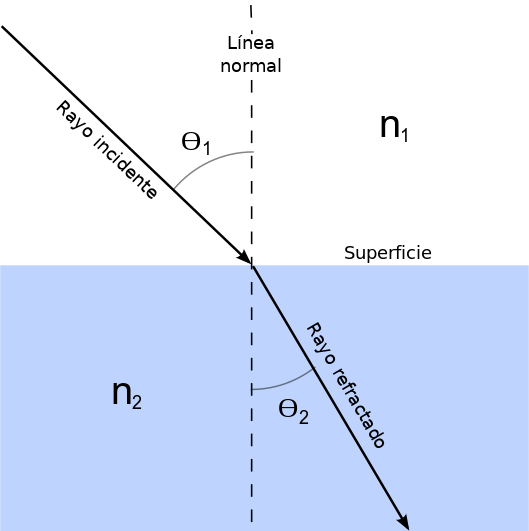
\includegraphics[width=0.6\linewidth]{Ant/Ant6.png}
\caption{Ley de Snell}
\end{figure}
dentro de ella una que usaremos es la del \textit{ángulo crítico}:
\begin{center}
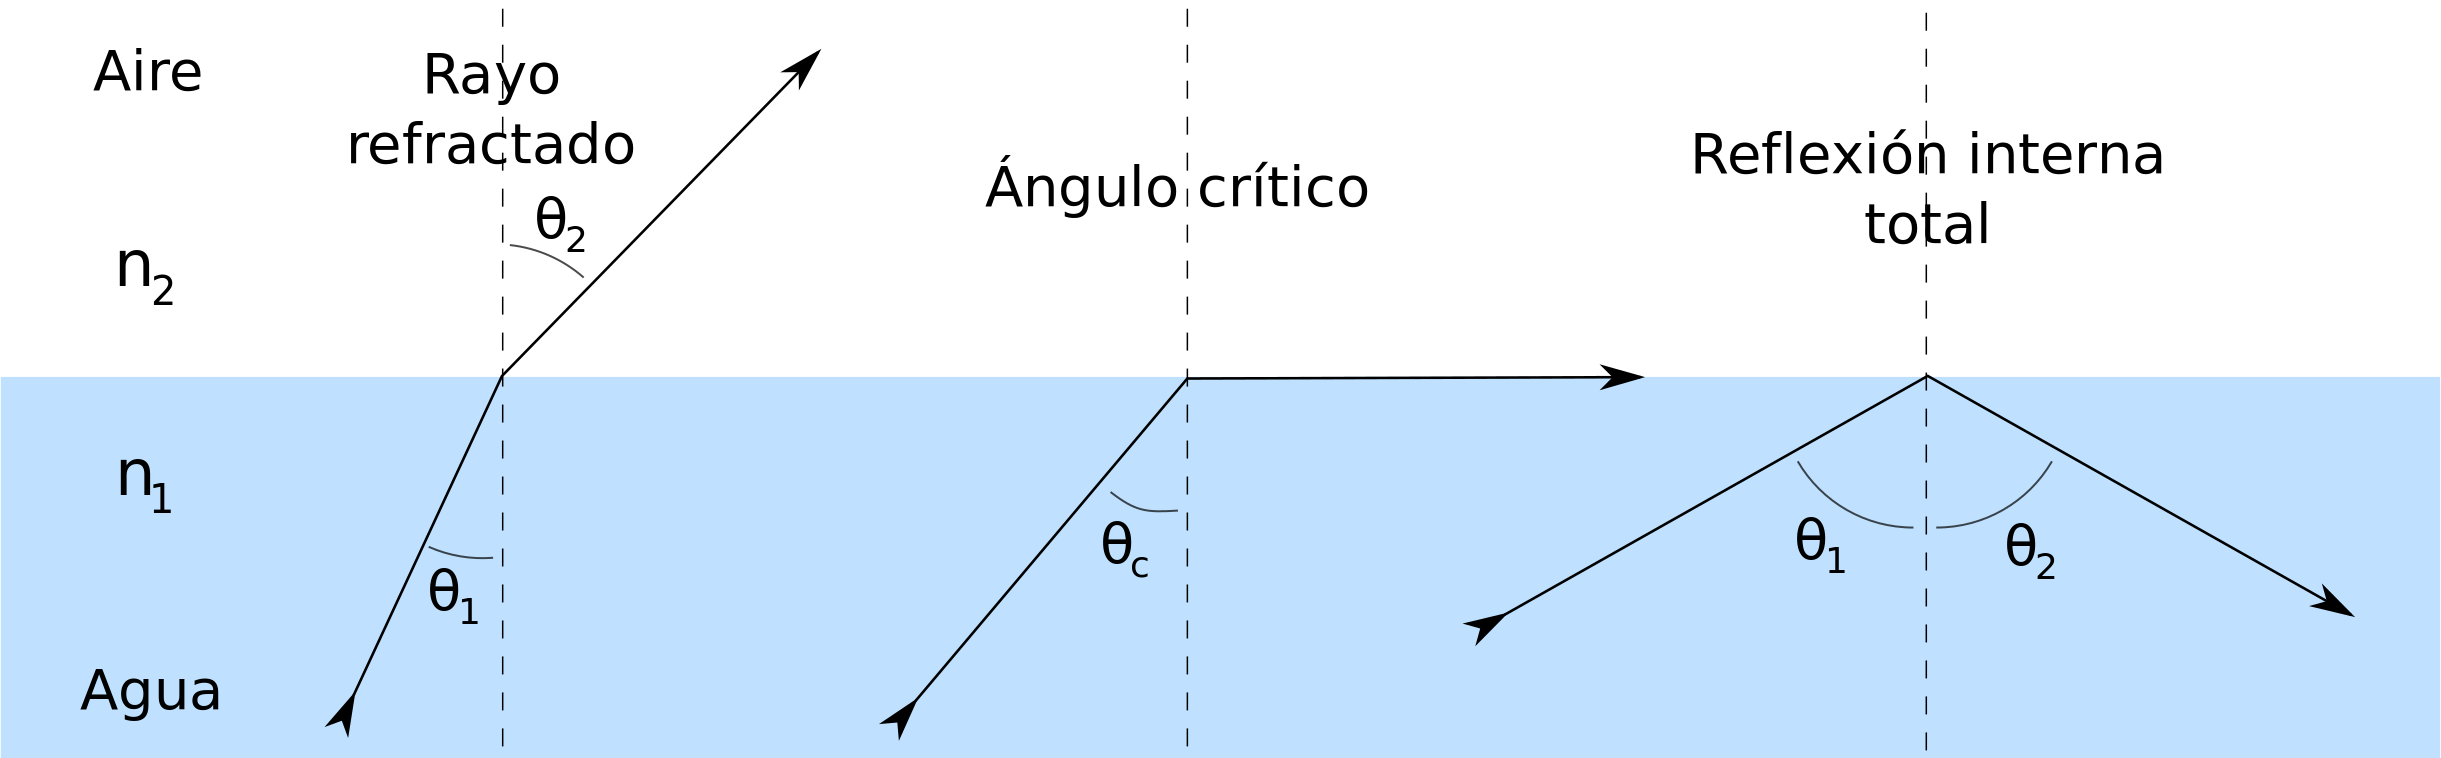
\includegraphics[width=0.8\linewidth]{Ant/Ant1.png}
\end{center}
La forma de obtener el ángulo crítico es:
\begin{equation}
\sin\theta_c=\frac{n_2}{n_1}
\label{eq: angulo critico}
\end{equation}
\begin{notation}
El índice de refracción esta definido como el cociente de la \textbf{velocidad de la luz en el vacío} entre la \textbf{velocidad de la luz del medio donde se propaga}. Generalmente se utiliza la velocidad de la luz en el vacío (\textit{c}) como medio de referencia para cualquier materia, aunque durante la historia se han utilizado otras referencias, como la velocidad de la luz en el aire. En el caso de la luz, es igual a $n=\sqrt{\epsilon_r\cdot\mu_r}$. Para la mayoría de los materiales, la \textbf{permeabilidad magnética relativa} ($\mu_r$) es muy cercano a 1 en frecuencias ópticas, es decir, luz visible, por lo tanto, \textit{n} es aproximadamente $\sqrt{\epsilon_r}$
\end{notation}
\subsection{Repaso: Propagación de ondas electromagnéticas}
La propagación de OEM por el espacio libre se suele llamar propagación de radiofrecuencia o radio propagación. Las OEM, en el espacio libre se propagan en línea recta a la velocidad de la luz ($3\basedec{8}m/s$). 
\begin{definition}[Distancia máxima de línea]
\begin{subequations}
\begin{align}
d_{max}&=\sqrt{2\cdot h}
\label{eq:dist millas} \\
d_{max}&=\sqrt{17\cdot h})\label{eq:dist km}
\end{align}
\end{subequations}
Donde:
\begin{itemize}
\item $d_{max}$: Distancia máxima de línea de vista. (millas ó Km)
\item \textbf{h}: Altura (Pies ó m)\footnote{La distancia será en millas si se trabaja con la ecuación \ref{eq:dist millas}, donde la altura debe ser introducida en pies. Para la ecuación \ref{eq:dist km}, la distancia estará en metros y la altura en metros.}
\end{itemize}
\end{definition}
Hablemos también de las \textbf{pérdidas por trayectoria}. El modelo de pérdida por trayectoria en el espacio libre es usado para predecir la intensidad del nivel de recepción cuando el transmisor y receptor tienen una trayectoria de línea de vista clara, sin obstrucciones entre ellos.
\begin{definition}[Pérdidas por trayectoria]
\begin{subequations}
\begin{align}
&L_p=\left(\frac{4\pi\cdot d}{\lambda}\right)^2=\left(\frac{4\pi\cdot d\cdot f}{c}\right)^2
\label{eq:perdidas trayec adimensional} \\
&L_p=20\cdot\log\left(\frac{4\pi\cdot d\cdot f}{c}\right)=20\cdot\log\left(\frac{4\pi}{c}\right)+20\cdot\log(f)+20\cdot\log(d)\label{eq:perdidas trayec db}
\end{align}
\end{subequations}
Donde:
\begin{itemize}
\item \textbf{d}: Distancia. (m)
\item \textbf{\textit{f}}: Frecuencia. (Hz)
\item \textbf{\textit{c}}: Velocidad de la luz.
\item $\lambda$: Longitud de onda. (m)
\end{itemize}
Si la distancia se expresa en Km y la frecuencia en MHz:
\begin{equation}
L_p(dB)=32.4+20\cdot\log(f)+20\log(d)
\end{equation}
\end{definition}
Otro término usado es la \textbf{polarización}, recordando que una OEM contiene un campo eléctrico y un campo magnético que forman 90° entre sí. Por lo tanto, la polarización de una OEM plana, no es mas que la orientación del vector campo eléctrico respecto a la superficie de la tierra.\\
\textbf{Tipos de polarización:}
\begin{enumerate}
\item \textbf{Polarización lineal}: Si la polarización permanece constante. Las formas lineales son:(Fig. \ref{fig:pol lin})
\begin{enumerate}
\item \textbf{Polarización Horizontal}: Campo eléctrico paralelo a la superficie de la tierra.
\item \textbf{Polarización Vertical}: Campo eléctrico perpendicular a la superficie terrestre.
\end{enumerate}
\item \textbf{Polarización Circular}: Luz polarizada circularmente consta de dos ondas electromagnéticas planas perpendiculares con una diferencia de fase de 90º. (Fig. \ref{fig:pol circ})
\item \textbf{Polarización elíptica}: La luz polarizada elípticamente consiste de dos ondas perpendiculares de amplitudes desiguales y con una diferencia de fase de 90º. (Fig. \ref{fig:pol elip})
\end{enumerate}
\begin{figure}[]
\centering
\subfloat[El campo eléctrico transversal de la onda va acompañado de un campo magnético como el que se ilustra.]{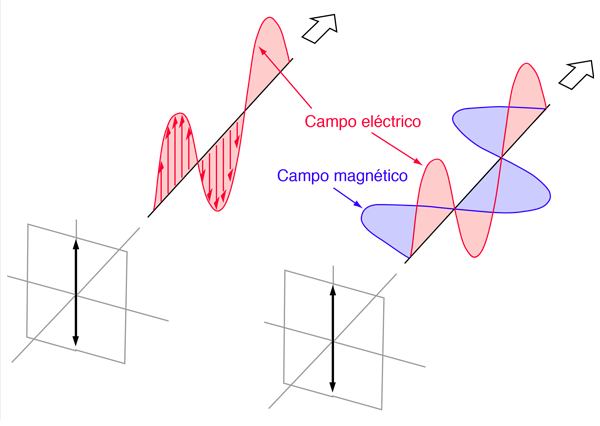
\includegraphics[width=0.5\linewidth]{Ant/Ant2.png}
\label{fig:pol lin}}
\subfloat[El vector de polarización gira 360º a medida de que la onda recorre una longitud de onda en el espacio]{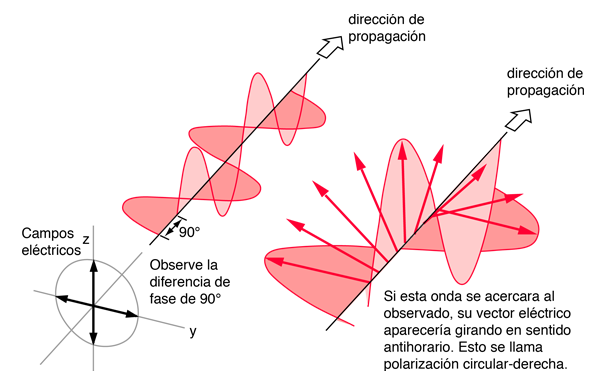
\includegraphics[width=0.5\linewidth]{Ant/Ant3.png}\label{fig:pol circ}}\\
\subfloat[Cuando la Intensidad de Campo varía con cambios en la polarización, se dice que es una Polarización Elíptica.]{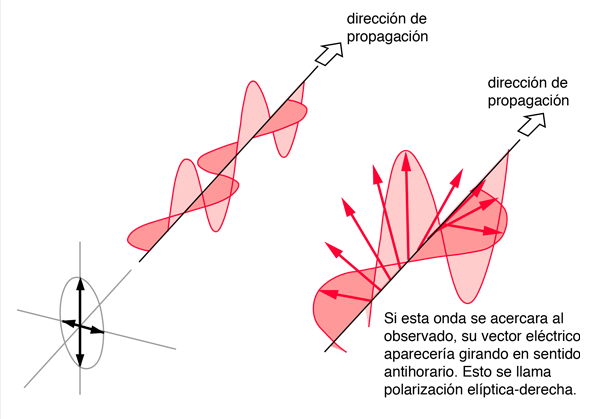
\includegraphics[width=0.5\linewidth]{Ant/Ant4.png}\label{fig:pol elip}}
\subfloat[Tipos de polarizaciones.]{
\includegraphics[width=0.5\linewidth]{Ant/Ant5.png}}
\caption{Polarización de ondas.}
\end{figure}
\begin{notation}
Si el vector gira en sentido de las manecillas del reloj, se dice que es Derecho, si es contrario se dice que es Izquierdo
\end{notation}
\subsubsection{Densidad de potencia radiada}
La \textbf{rapidez} con que la energía pasa a través de una \textbf{superficie} dada en el espacio libre se llama D\textbf{ensidad de Potencia}. La \textbf{Densidad de Potencia Radiada} se define como la potencia por unidad de superficie en una determinada dirección. Las unidades son \textbf{Watt por Metro Cuadrado} ($W/m^2$). Se puede calcular a partir de los valores eficaces de los campos eléctrico o magnéticos.
\begin{definition}[Potencia Isotrópica Radiada Equivalente]
\begin{equation}
PIRE=P_r\cdot D=P_A\cdot G
\label{eq:pire}
\end{equation}
Donde:
\begin{itemize}
\item PIRE:  Potencia Isotrópica Radiada Equivalente. (W)
\item $P_R$: Potencia de radiación.
\item $P_A$: Potencia suministrada a la antena. (W)
\item \textbf{G}: Ganancia.
\item \textbf{D}: Directividad de la antena.\footnote{Estos conceptos se detallan más adelante.}
\end{itemize}
\end{definition}
\begin{definition}[Intensidad de campo]
Es la intensidad de los campos eléctrico y magnético de una onda electromagnética que se propaga por el espacio libre.
\begin{equation}
\mathbb{P}=E\cdot H=\frac{PIRE}{4\pi r^2}=Z_s\times H^2=\frac{E^2}{Z_s}
\label{eq:int campo}
\end{equation}
Donde:
\begin{itemize}
\item $\mathbb{P}$: Densidad de potencia. ($W/m^2$)
\item \textbf{E}: Intensidad de campo eléctrico. (V/m)
\item \textbf{H}: Intensidad del campo magnético. (A/m)
\item \textbf{r}: Radio de la esfera. (m)
\item \textbf{\textit{PIRE}}: Potencia Isotrópica Radiada Equivalente. (W)
\end{itemize}

\end{definition}
\begin{definition}[Impedancia en el espacio libre]
La relación entre el módulo del campo eléctrico y el módulo del campo magnético es la impedancia característica del medio. La impedancia característica de un medio de transmisión \textbf{sin pérdidas} en igual a la raíz cuadrada de la relación de su permeabilidad magnética entre su permitividad eléctrica:
\begin{equation}
Z_s=\sqrt{\frac{\mu_0}{\epsilon_0}}=377\Omega
\label{eq:imp carac espacio libre}
\end{equation}
Donde:
\begin{itemize}
\item $Z_s$: Impedancia en el espacio libre. ($\Omega$)
\item $\mu_0$: Permeabilidad magnética ($1.26\basedec{-6}$H/m ó $4\pi\cdot K N/A^2$ donde $K=\basedec{-7}$).
\item $\epsilon_0$: Permitividad eléctrica del vacío ($8.85\basedec{-12}$F/m).
\end{itemize}
\end{definition}
%\begin{definition}[Potencia total radiada]
%Se puede obtener como la integral de la Densidad de Potencia en una esfera que encierre a la antena.
%\begin{equation}
%P_{tr}=\frac{P_{rad}}{4\pi r^2}
%\end{equation}
%\end{definition}
La \textbf{Intensidad de Radiación} es la potencia radiada por unidad de ángulo sólido en una determinada dirección.
\subsubsection{Ley de cuadrado inverso}
La \textbf{densidad de potencia} es inversamente proporcional al cuadrado de la distancia de la fuente.
\begin{equation}
\frac{\mathbb{P}_2}{\mathbb{P}_1}=\left(\frac{r_1}{r_2}\right)^2
\label{eq:ley cuadrado inverso}
\end{equation}
Para que se cumpla esta ley, la velocidad de propagación en todas las direcciones debe ser uniforme (Medio Isotrópico)
\subsubsection*{Atenuación y absorción}
\textbf{Atenuación} es la reducción de la Densidad de Potencia con la distancia. La atenuación se debe al esparcimiento esférico de la onda, se le llama ``atenuación espacial'' de la onda. Se expresa generalmente en términos del logaritmo de la relación de  densidad de  potencia (pérdida en dB)\\
\textbf{Absorción} solo se presenta cuando los CEM se propagan por la atmósfera. Es la energía transferida de la OEM a los átomos y las moléculas de la atmósfera. La absorción de radiofrecuencias en una atmósfera normal, es relativamente insignificante a frecuencias por debajo de 10 GHz.
\section{Antenas}
Las dos funciones primordiales de la antena son:
\begin{enumerate}
\item Convertir la energía electromagnética, procedente del generados a través de la línea de transmisión, en energía electromagnética que se propaga libremente por el espacio.
\item Adapta la impedancia interna del generador a la impedancia del espacio.
\end{enumerate}
En las líneas de transmisión se propagan ondas electromagnéticas \textbf{guiadas}, es decir campos electromagnéticos variables entre cargas y corrientes. Las antenas convierten estos ondas electromagnéticas guiadas en \textbf{libres} y \textbf{viceversa}. Tanto las ondas guiada como las libres son señales de radio.\\
En el proceso de su propagación, las ondas de radio se \textbf{dispersan} más allá de las líneas de radio-comunicación y son absorbidas por el medio circundante. Si la dirección de radiocomunicación es conocida y limitada, las perdidas pueden reducirse concentrando las ondas emitidas en direcciones definidas.\\
Con lo definido sobre antenas y conocimientos en impedancias, podemos definir:
\begin{corollary}[Impedancia de antena]
Es la relación entre tensión y corriente en sus terminales de entrada (de la antena). Como todas, dicha impedancia es en general compleja: parte real ó resistencia de antena y la parte compleja ó reactancia de antena.
\end{corollary}
\subsection{Tipos de antenas}
A grandes rasgos existen dos tipos de antenas: antenas de \textbf{transmisión} y antenas de \textbf{recepción}.
\subsubsection*{Antenas de transmisión}
La antena de transmisión transforma energía de un campo electromagnético estacionario producido por la señal de radio, en energía de un campo electromagnético de radiación, añadiendo además que este último debe emitirse en unas direcciones dadas.
\begin{figure}[]
\centering
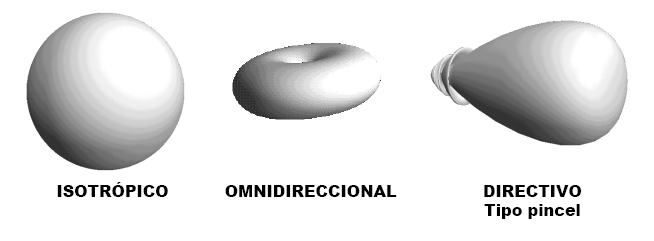
\includegraphics[width=0.8\linewidth]{Ant/Ant7.png}
\caption{Gráficas de antena.}
\end{figure}
\subsubsection*{Antenas de recepción}
La antena de recepción está destinada a la transformación de la energía de una radioseñal consistente en un campo de radiación que procede de una dirección dada, en energía de un campo estacionario de ondas electromagnéticas.
\begin{remark}
La antena de transmisión y recepción tienen procesos \textbf{recíprocos}. Esto quiere decir que existe la posibilidad de utilizar la misma antena en calidad de transmisora y de receptora, y de conservar invariables los parámetros principales de la antena.
\end{remark}
\subsection{Características y parámetros de las antenas transmisoras}
Los parámetros de una antena son los que permiten especificar el funcionamiento de las mismas, y por lo tanto son susceptibles de ser medidos. Se puede especificar la antena como un \textbf{conjunto de parámetros} conectados con los  requisitos de un sistema más amplio de radiocomunicaciones o radiodifusión.\\
\textbf{Parámetros de antena}:
\begin{itemize}
\item Diagrama de radiación
\item Densidad de potencia radiada
\item Directividad
\item Ganancia
\item Polarización
\item Impedancia
\item Adaptación
\item Área y longitud efectiva
\end{itemize}
\begin{definition}[Potencia de radiación y resistencia de radiación]
Representa la característica de la antena para la emisión energía electromagnética.
\begin{equation}
R_r=\frac{P_r}{i^2}
\label{eq:resistencia radiacion}
\end{equation}
Donde:
\begin{itemize}
\item $R_r$: Resistencia de total de radiación. ($\Omega$)
\item $P_r$: Potencia de radiación. (W)
\item \textbf{i}: Valor eficaz de la corriente de la antena. (A)
\end{itemize}
\end{definition}
Cuantitativamente la resistencia de radiación de define como aquella resistencia pura en la que se libera una potencia numéricamente igual a la potencia de radiación, para una corriente en la resistencia igual ala corriente en la antena.
\begin{definition}[Potencia de Pérdidas y resistencia de pérdidas]
Potencia que se pierde por el calentamiento del conductor, en los aisladores, en la tierra y en los objetos situados cerca de la antena.
\begin{equation*}
R_p=\frac{P_p}{i^2}
\label{eq:resistencia perdidas}
\end{equation*}
Donde:
\begin{itemize}
\item $R_p$: Resistencia de pérdidas. ($\Omega$)
\item $P_p$: Potencia de pérdidas. (W)
\item \textbf{i}: Valor eficaz de la corriente de la antena. (A)
\end{itemize}
\end{definition}
\begin{definition}[Potencia de una antena y resistencia activa total o resistencia de antena]
Resistencia que corresponde a potencia suministrada a la antena. Potencia de antena es la suministrada a la antena por el transmisor, a través de la línea de transmisión, se obtiene con la suma de la potencia de \textbf{radiación} y la potencia de \textbf{pérdidas}.
\begin{equation}
P_A=P_r+P_p=i^2\left(R_r+R_p\right)
\label{eq:potencia antena}
\end{equation}
\begin{equation}
R_A=R_r+R_p
\end{equation}
Donde:
\begin{itemize}
\item $P_A$: Potencia suministrada a la antena. (W)
\item $P_r$: Potencia de radiación. (W)
\item $P_p$: Potencia de pérdidas. (W)
\item \textbf{i}: Valor eficaz de la corriente de la antena. (A)
\item $R_r$: Resistencia de radiación. ($\Omega$)
\item $R_p$: Resistencia de pérdidas. ($\Omega$)
\item $R_A$: Resistencia activa total. ($\Omega$)
\end{itemize}
\end{definition}
\begin{definition}[Rendimiento o Eficacia de una antena]
Es la relación entre la Potencia de Radiación y la Potencia Suministrada a la Antena.
\begin{equation*}
\eta_A=\frac{P_r}{P_A}=\frac{R_r}{R_r+R_p}=\frac{R_r}{R_A}=\frac{G}{D}
\label{eq:rendimiento de antena}
\end{equation*}
\begin{displaymath}
0\leq\eta_A\leq 1
\end{displaymath}
Donde:
\begin{itemize}
\item $\eta_A$: Rendimiento de antena.
\item $P_A$: Potencia suministrada a la antena. (W)
\item $P_r$: Potencia de radiación. (W)
\item $R_r$: Resistencia de radiación. ($\Omega$)
\item $R_p$: Resistencia de pérdidas. ($\Omega$)
\item $R_A$: Resistencia activa total. ($\Omega$)
\item \textbf{G}: Ganancia.
\item \textbf{D}: Directividad.
\end{itemize}
\end{definition}
\subsection{Parámetros de acción directiva de antenas}\index{Parámetros de acción directiva de antenas}
\subsubsection{Directividad}
La característica de directividad de antena muestra la \textbf{dependencia} de la intensidad de campo de radiación respecto a la dirección, con la condición que este campo sea medido siempre a igual distancia de la antena. Para el estudio de la radiación de una antena, se supone que la antena está situada en el punto medio de una ``esfera'' y en el origen de un sistema de coordenadas espaciales.
En la superficie de la ``esfera'' se calcula E y H en cualquier punto de esta, alejado una distancia \textit{r} del centro del dipolo.\\
\textbf{Características:}
\begin{enumerate}
\item \textbf{Propiedad Directiva}: Todas las antenas reales tienden a concentrar los campos radiado en alguna dirección.
\item \textbf{Característica de Directividad}: Depende de la intensidad de campo de radiación, respecto a la dirección, medido siempre a igual distancia de la antena. 
\item \textbf{Función de Directividad}: Expresión matemática de la directividad.
\begin{displaymath}
f^2(\theta,\phi)
\end{displaymath}
\item \textbf{Diagrama de Directividad}: Representación gráfica de la función de directividad. Normalmente se expresa en proyecciones:
\begin{enumerate}
\item Plano Horizontal ( $\phi$ varía y $\theta$ = 90º)
\item Plano Vertical ( $\theta$ varía y $\phi$	 = 0º)
\end{enumerate}
\end{enumerate}
\begin{definition}[Factor de directividad]
Factor de Directividad es la relación entre la densidad del flujo de potencia emitido por la antena dada en una \textbf{determinada dirección}, y la densidad de flujo de potencia que emitiría una antena absolutamente \textbf{no direccional} en cualquier dirección, siendo iguales las potencias totales de radiación de ambas antenas y medido a igual distancia.
\begin{equation}
D=\frac{\mathbb{P}_{max}}{\mathbb{P}_{ref}}=\frac{E_{max}^2}{E_0^2}
\label{eq:directividad}
\end{equation}
Donde:
\begin{itemize}
\item \textbf{D}: Factor de directividad.
\item $\mathbb{P}_{max}$: Densidad de potencia en un punto, en la dirección de máxima radiación. ($W/m^2$)
\item $\mathbb{P}_{ref}$: Densidad de potencia en el mismo punto, con una antena no direccional o de referencia. ($W/m^2$)
\end{itemize}
\end{definition}
\begin{figure}[H]
\centering
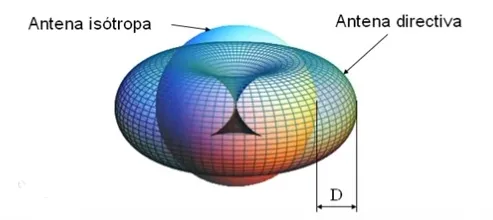
\includegraphics[width=0.7\linewidth]{Ant/Ant8.png}
\caption{Representación tridimensional de la directividad.}
\end{figure}
\begin{definition}[Ganancia de potencia]
\begin{equation}
G=\eta_A\cdot D=\frac{\mathbb{P}_{max}}{\mathbb{P}_{ref}'}
\label{eq:ganancia}
\end{equation}
Donde:
\begin{itemize}
\item \textbf{G}: Ganancia.
\item $\eta_A$: Rendimiento de la antena.
\item \textbf{D}: Directividad de la antena.
\item $\mathbb{P}_{max}$: Densidad de potencia en un punto, en la dirección de máxima radiación. ($W/m^2$)
\item $\mathbb{P}_{ref}'$: Densidad de potencia en el mismo punto, con una antena no direccional o de referencia sin pérdidas. ($W/m^2$)
\end{itemize}
\end{definition}
\begin{definition}[Factor de calidad]
\begin{equation}
Q=\frac{f_r}{BW}
\label{eq:factor de calidad}
\end{equation}
Donde:
\begin{itemize}
\item Q: Factor de calidad.
\item $f_r$: Frecuencia de resonancia. (Hz)
\item $BW$: Ancho de banda. (Hz)
\end{itemize}
\end{definition}
\subsection{Antenas receptoras}
\begin{definition}[Área de captura]
Mientras que la \textbf{ganancia de potencia} es el parametro natural para describir la mayor densidad de potencia de una señal transmitida, por las propiedades direccionales de la antena transmisora, para describir las propiedades receptiras de una antena se usa una cantidad relacionada: \textbf{área de captura}
\begin{equation}
A_{cap}=\frac{G_r\cdot\lambda^2}{4\pi}
\label{eq:area capturada}
\end{equation}
Donde:
\begin{itemize}
\item $A_{cap}$: Área efectiva de captura. ($m^2$)
\item $G_r$: Ganancia del receptor.
\item $\lambda$: Longitud de onda de la señal recibida. (m)
\end{itemize}
\end{definition}
\begin{definition}[Potencia capturada]
Potencia disponible en las terminales de salida de la antena receptora. La potencia capturada es directamente proporcional a la densidad de potencia recibida y al área de captura de la antena receptora.
\begin{equation}
P_{cap}=\mathbb{P}\cdot A_{cap}\cdot G
\label{eq:potencia capturada}
\end{equation}
Donde:
\begin{itemize}
\item $P_{cap}$: Potencia capturada. (W)
\item $\mathbb{P}$: Densidad de potencia capturada. ($W/m^2$)
\item $A_{cap}$: Área capturada. ($m^2$)
\item \textbf{G}: Ganancia.
\end{itemize}
\end{definition}
\begin{remark}
Recuerda que en todas las ecuaciones se debe trabajar con unidades \textbf{lineales}. Esto significa que todos los decibelios que nos da los problemas deben ser transformadas a sus equivalentes lineales para poder usar las ecuaciones dadas a los largo de este capitulo.
\end{remark}
%----------------------------------------------------------------------------------------
%	NEW CHAPTER
%----------------------------------------------------------------------------------------
\part{Internetworking 2}
\chapterimage{chapter_head_IT2.pdf} % Chapter heading image

\chapter{Unidad I}
\section{Protocolo spanning tree}\index{Protocolo spanning tree}
Las redes conmutadas, por lo general, tienen rutas  redundantes y enlaces redundantes incluso entre los  mismos dos dispositivos. Las rutas redundantes eliminan un punto de falla único  para mejorar la confiabilidad y disponibilidad. Las rutas redundantes pueden causar bucles de capa 2  físicos y lógicos.
\begin{figure}[H]
\centering
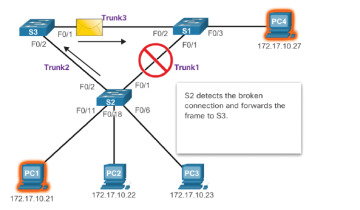
\includegraphics[width=0.6\linewidth]{IN2/IN1.png}
\caption{Camino redundante de PC1 a PC4 en caso falle una ruta.}
\end{figure}
El algoritmo \textbf{Spanning Tree} (árbol de expansión) se utiliza en los switches para prevenir los bucles lógicos que pueden aparecer en una red. Los bucles se producen cuando existen varios caminos distintos entre dos puntos de la red y su efecto es que las tramas pueden circular de forma indefinida atrapadas en un bucle sin conseguir alcanzar su destino, lo que además afectará negativamente al rendimiento de la red. El algoritmo \textit{Spanning Tree} ayuda a los switches a elegir el camino más idóneo y, por tanto, elimina los bucles.
\begin{notation}
El protocolo \textit{spanning tree esta detallado especificado en el estándar \textbf{IEEE 802.1D}. Existe su variante con funcionamiento optimizado: \textbf{spanning tree rápido}-IEEE 802.1w}
\end{notation}
\subsection{Problemas con la redundancia de capa 1}
Los problemas con los bucles son:
\begin{itemize}
\item \textbf{Inestabilidad de la base de datos MAC}: Las tramas de ethernet no poseen Tiempo de duración, como el encabezado IP de capa 3. Esto significa que Ethernet no tiene ni un mecanismo para descartar las tramas que se propagan innecesariamente. EL bucle empieza de la siguiente manera; observando la imagen  \ref{fig:inestabilidad spanning tree}:
\begin{enumerate}
\item PC1 envía un marco de transmisión a S2. S2 recibe el marco de transmisión en F0/11. Cuando S2 recibe la trama de transmisión, actualiza su tabla de direcciones MAC para registrar que la PC1 está disponible en el puerto F0/11.
\item Debido a que es una trama de transmisión, S2 reenvía la trama por todos los puertos, incluidos Trunk1 y Trunk2. Cuando la trama de transmisión llega a S3 y S1, los switches actualizan sus tablas de direcciones MAC para indicar que PC1 está disponible en el puerto F0/1 en S1 y en el puerto F0/2 en S3.
\item Debido a que es una trama de transmisión, S3 y S1 reenvían la trama por todos los puertos excepto el puerto de entrada. S3 envía el marco de transmisión de PC1 a S1. S1 envía el marco de transmisión de PC1 a S3. Cada conmutador actualiza su tabla de direcciones MAC con el puerto incorrecto para PC1.
\item Cada conmutador reenvía la trama de difusión por todos sus puertos excepto el puerto de entrada, lo que hace que ambos conmutadores reenvíen la trama a S2.
\item Cuando S2 recibe las tramas de transmisión de S3 y S1, la tabla de direcciones MAC se actualiza con la última entrada recibida de los otros dos conmutadores.
\item S2 reenvía la trama de transmisión por todos los puertos excepto el último puerto recibido. El ciclo comienza de nuevo.
\end{enumerate}
\begin{figure}[H]
\centering
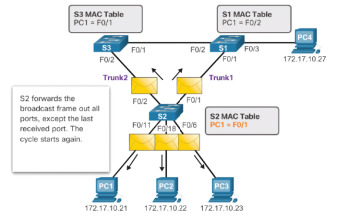
\includegraphics[width=0.6\linewidth]{IN2/IN2.png}
\caption{Momento 6 del bucle.}
\label{fig:inestabilidad spanning tree}
\end{figure}
Debido a los cambios constantes en la tabla de direcciones MAC, los switches S3  y S1 no saben a qué puerto reenviar las tramas.
\item \textbf{Tormenta de difusión}: Si no controlamos el problema anterior, las demás computadoras también deben mandar primero sus marcos de transmisión, y el problema de inestabilidad se acrecentará, esto se refleja en el sistema como varios tramas de transmisión \textbf{atrapados} en la red, \textbf{consumiendo ancho de banda} y hasta saturándola. Haciendo que sea imposible el envío de datos legítimos de comunicación. Si no hay ancho de banda útil para el envío de información, la red no estará disponible causando una denegación de servicio efectiva (DoS).\\
Hay otras consecuencias de las tormentas de transmisión. Debido a que el tráfico de difusión se reenvía a todos los puertos de un conmutador, todos los dispositivos conectados tienen que procesar todo el tráfico de difusión que se inunda sin cesar alrededor de la red en bucle. Esto puede hacer que el dispositivo final no funcione correctamente debido a los requisitos de procesamiento necesarios para soportar una carga de tráfico tan alta en la NIC.\\
Secuencia de eventos:
\begin{enumerate}
\item PC1 envía una trama de transmisión a la red en bucle (Inestabilidad en la base de datos MAC).
\item La trama de transmisión se repite entre todos los conmutadores interconectados en la red.
\item La PC4 también envía una trama de transmisión a la red en bucle.
\item La trama de transmisión PC4 queda atrapada en el bucle entre todos los conmutadores interconectados, al igual que la trama de transmisión PC1.
\item A medida que más dispositivos envían transmisiones a través de la red, más tráfico queda atrapado en el bucle y consume recursos. Esto eventualmente crea una tormenta de transmisión que hace que la red falle.
\item Cuando la red está totalmente saturada con el tráfico de difusión que circula entre los conmutadores, el conmutador descarta el tráfico nuevo porque no puede procesarlo. La Figura \ref{fig:tormenta de difusión} muestra la tormenta de difusión resultante.
\end{enumerate}
\begin{figure}[H]
\centering
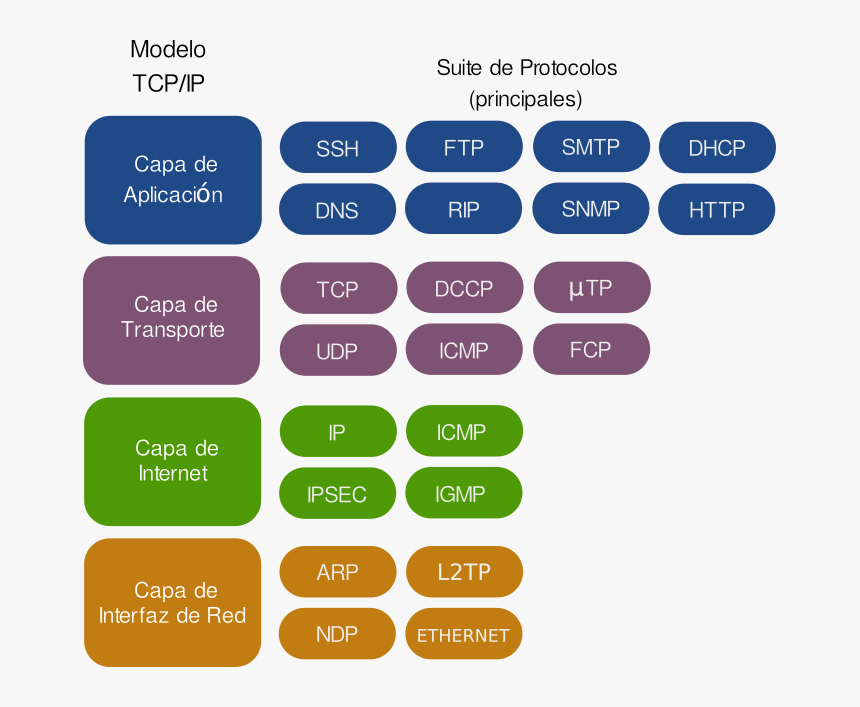
\includegraphics[width=0.6\linewidth]{IN2/IN3.png}
\caption{Tormenta de difusión}
\label{fig:tormenta de difusión}
\end{figure}
Una tormenta de transmisión puede desarrollarse en segundos porque los dispositivos conectados a una red envían regularmente tramas de transmisión, como solicitudes ARP. Como resultado, cuando se crea un bucle, la red conmutada se desconecta rápidamente.
\item \textbf{Tramas de unidifusión duplicadas}: Una trama de unidifusión desconocida se produce  cuando el switch no tiene la dirección MAC de destino en la tabla de direcciones MAC y debe difundir la trama a todos los puertos, excepto el  puerto en que se recibió la trama (puerto de ingreso). Si se envían tramas de unidifusión desconocidas a  una red con bucles, se puede producir la llegada de  tramas duplicadas al dispositivo de destino.\\
Secuencia de eventos:
\begin{enumerate}
\item PC1 envía una trama de unidifusión destinada a PC4.
\item S2 no tiene una entrada para PC4 en su tabla MAC. En un intento por encontrar la PC4, inunda la trama de unidifusión desconocida de todos los puertos del switch excepto el puerto que recibió el tráfico.
\item La trama llega a los conmutadores S1 y S3.
\item S1 tiene una entrada de dirección MAC para PC4, por lo que reenvía la trama a PC4.
\item S3 tiene una entrada en su tabla de direcciones MAC para PC4, por lo que reenvía la trama de unidifusión de Trunk3 a S1.
\item S1 recibe la trama duplicada y la reenvía a la PC4.
\item PC4 ahora ha recibido el mismo marco dos veces.
\end{enumerate}
\begin{figure}[H]
\centering
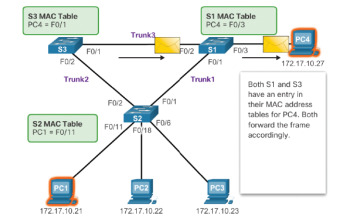
\includegraphics[width=0.6\linewidth]{IN2/IN4.png}
\caption{S1 y S3 envian una trama duplicada a la PC4.}
\end{figure}
\end{itemize}
\subsection{Introducción}

\section{Tecnología EtherChannel}
\subsection{Funcionamiento}
Hay escenarios en los que se necesita más ancho de banda o redundancia entre  dispositivos que lo que puede proporcionar un único enlace. Se pueden conectar varios  enlaces entre dispositivos para aumentar el ancho de banda. Sin embargo, el protocolo de  árbol de expansión (STP), que está habilitado en dispositivos de \textbf{capa 2} como switches. Cisco de forma predeterminada, bloqueará enlaces redundantes para evitar bucles de  conmutación. Se necesita una tecnología de agregación de enlaces que permita \textbf{vínculos redundantes} entre dispositivos que \textbf{no serán bloqueados por STP}. Esa tecnología se conoce como EtherChannel.\\
EtherChannel es una tecnología de agregación de enlaces que \textbf{agrupa} varios enlaces físicos Ethernet en un único enlace lógico. Se utiliza para proporcionar tolerancia a fallos, uso compartido de carga, mayor ancho de banda y redundancia entre switches, routers y servidores. La tecnología de EtherChannel hace posible combinar la cantidad de enlaces físicos entre los switches para aumentar la velocidad general de la comunicación switch a switch.\\
En los inicios, Cisco desarrolló la  tecnología EtherChannel como una técnica switch a switch LAN  para \textbf{agrupar} varios puertos Fast  Ethernet o gigabit Ethernet en un  único canal lógico. Cuando se configura un EtherChannel, la interfaz virtual  resultante se denomina ``canal de  puertos'' (\textit{port channel}). Las interfaces físicas se agrupan en una interfaz de canal  de puertos, como se muestra en la figura \ref{fig:tec ether}.
\begin{figure}[H]
\centering
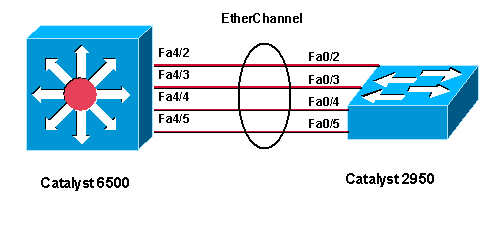
\includegraphics[width=0.6\linewidth]{IN2/IN5.png}
\caption{Tecnología EtherChannel}
\label{fig:tec ether}
\end{figure}
\subsection{Ventajas de EtherChannel}
\begin{itemize}
\item La mayoría de las tareas de configuración se pueden realizar en la interfaz EtherChannel en lugar  de en cada puerto individual, lo que asegura la coherencia de configuración en todos los enlaces.
\item EtherChannel depende de los puertos de switch existentes. No es necesario actualizar el enlace a  una conexión más rápida y más costosa para tener más ancho de banda.
\item El equilibrio de carga ocurre entre los enlaces que forman parte del mismo EtherChannel.
\item EtherChannel crea una agregación que se ve como un único enlace lógico. Cuando existen varios  grupos EtherChannel entre dos switches, STP puede bloquear uno de los grupos para evitar los  bucles de switching. Cuando STP bloquea uno de los enlaces redundantes, bloquea el  EtherChannel completo. Esto bloquea todos los puertos que pertenecen a ese enlace  EtherChannel. Donde solo existe un único enlace EtherChannel, todos los enlaces físicos en el  EtherChannel están activos, ya que STP solo ve un único enlace (lógico).
\item EtherChannel proporciona redundancia, ya que el enlace general se ve como una única conexión  lógica. Además, la pérdida de un enlace físico dentro del canal no crea ningún cambio en la  topología.
\end{itemize}
\subsection{Restricciones}
\begin{itemize}
\item No pueden mezclarse los tipos de interfaz. Por ejemplo, Fast Ethernet y Gigabit Ethernet no se pueden mezclar dentro de un único EtherChannel.
\item En la actualidad, cada EtherChannel puede constar de hasta ocho puertos Ethernet configurados  de manera compatible. El EtherChannel proporciona un ancho de banda full-duplex de hasta 800  Mbps (Fast EtherChannel) u 8 Gbps (Gigabit EtherChannel) entre un switch y otro switch o host.
\item El switch Cisco Catalyst 2960 Layer 2 soporta actualmente hasta seis EtherChannels.
\item La configuración de los puertos individuales que forman parte del grupo EtherChannel debe ser  coherente en ambos dispositivos. Si los puertos físicos de un lado se configuran como enlaces  troncales, los puertos físicos del otro lado también se deben configurar como enlaces troncales  dentro de la misma VLAN nativa. Además, todos los puertos en cada enlace EtherChannel se  deben configurar como puertos de capa 2.
\item Cada EtherChannel tiene una interfaz de canal de puertos lógica, la configuración aplicada a la  interfaz de canal de puertos afecta a todas las interfaces físicas que se asignan a esa interfaz.
\end{itemize}
\subsection*{Protocolos de negociación automática}
Los EtherChannels se pueden formar por medio de una negociación con uno de dos  protocolos: Port Aggregation Protocol (PAgP) o Link Aggregation Control Protocol (LACP).  Estos protocolos permiten que los puertos con características similares formen un canal  mediante una negociación dinámica con los switches adyacentes.
\subsection{Funcionamiento del PAgP}
PAgP (pronunciado ``Pag - P'') es un protocolo patentado por Cisco que ayuda en la creación  automática de enlaces EtherChannel. Cuando se configura un enlace EtherChannel mediante PAgP,  se envían paquetes PAgP entre los puertos aptos para EtherChannel para negociar la formación de un  canal. Cuando PAgP identifica enlaces Ethernet compatibles, agrupa los enlaces en un EtherChannel.  El EtherChannel después se agrega al árbol de expansión como un único puerto.\\
Cuando se habilita, PAgP también administra el EtherChannel. Los paquetes PAgP se envían cada 30  segundos. PAgP revisa la coherencia de la configuración y administra los enlaces que se agregan, así  como las fallas entre dos switches. Cuando se crea un EtherChannel, asegura que todos los puertos  tengan el mismo tipo de configuración.
\begin{notation}
En EtherChannel, es obligatorio que todos los puertos tengan la misma velocidad, la misma  configuración de dúplex y la misma información de VLAN. Cualquier modificación de los puertos  después de la creación del canal también modifica a los demás puertos del canal.
\end{notation}
\subsection{PAgP}\index{PAgP}
PAgP ayuda a crear el enlace EtherChannel al detectar la configuración de cada lado y asegurarse de que los enlaces sean  compatibles, de modo que se pueda habilitar el enlace EtherChannel cuando sea necesario. Los modos de PAgP de la siguiente  manera:
\begin{itemize}
\item \textbf{Encendido}: Este modo obliga a la interfaz a proporcionar un canal sin PAgP. Las interfaces configuradas en el modo encendido no intercambian paquetes PAgP.
\item \textbf{PAgP desirable}: Este modo PAgP coloca una interfaz en un estado de negociación activa en el que la interfaz inicia negociaciones con otras interfaces al enviar paquetes PAgP.
\item \textbf{PAgP auto}: Este modo PAgP coloca una interfaz en un estado de negociación pasiva en el que la interfaz responde a los paquetes PAgP que recibe, pero no inicia la negociación PAgP.
\end{itemize}
Los modos deben ser compatibles en cada lado. Si se configura un lado en modo automático, se coloca en estado pasivo, a la  espera de que el otro lado inicie la negociación del EtherChannel. Si el otro lado se establece en modo automático, la  negociación nunca se inicia y no se forma el canal EtherChannel. Si se deshabilitan todos los modos mediante el comando \textit{\textbf{no}} o  si no se configura ningún modo, entonces se deshabilita el EtherChannel. El modo \textit{encendido} coloca manualmente la interfaz en  un EtherChannel, sin ninguna negociación. Funciona solo si el otro lado también se establece en modo encendido. Si el otro lado  se establece para negociar los parámetros a través de PAgP, no se forma ningún EtherChannel, ya que el lado que se establece  en modo \textit{encendido} no negocia. El hecho de que no haya negociación entre los dos switches significa que no hay un control, para asegurarse de que todos los enlaces en el EtherChannel terminen del otro lado o de que haya compatibilidad con PAgP en  el otro switch.
\begin{table}[H]
\centering
\begin{tabular}{|c|c|c|}
\hline
\rowcolor[HTML]{9698ED} 
S1        & S2             & Establecmiento del canal \\ \hline
On        & On             & Sí                       \\ \hline
On        & Desirable/Auto & No                       \\ \hline
Desirable & Desirable      & Sí                       \\ \hline
Desirable & Auto           & Sí                       \\ \hline
Auto      & Desirable      & Sí                       \\ \hline
Auto      & Auto           & No                       \\ \hline
\end{tabular}
\caption{Combinacion PAgP y el resultado del establecimiento.}
\end{table}
\subsection{LACP}\index{LACP}
LACP forma parte de una especificación \textbf{IEEE (802.3ad)} que permite agrupar varios puertos físicos  para formar un único canal lógico. LACP permite que un switch negocie un grupo automático mediante  el envío de paquetes LACP al otro switch. Realiza una función similar a PAgP con EtherChannel de  Cisco. Debido a que LACP es un estándar IEEE, se puede usar para facilitar los EtherChannels en entornos de varios proveedores. En los dispositivos de Cisco, se admiten ambos protocolos.\\
LACP proporciona los mismos beneficios de negociación que PAgP. LACP ayuda a crear el enlace  EtherChannel al detectar la configuración de cada lado y al asegurarse de que sean compatibles, de  modo que se pueda habilitar el enlace EtherChannel cuando sea necesario. Los modos para LACP  son los siguientes:
\begin{itemize}
\item \textbf{On}: Este modo obliga a la interfaz a proporcionar un canal sin LACP. Las interfaces
configuradas en el modo encendido no intercambian paquetes LACP.
\item \textbf{LACP active}: Este modo de LACP coloca un puerto en estado de negociación activa. En este
estado, el puerto inicia negociaciones con otros puertos mediante el envío de paquetes LACP.
\item \textbf{LACP passive}: Este modo de LACP coloca un puerto en estado de negociación pasiva. En este  estado, el puerto responde a los paquetes LACP que recibe, pero no inicia la negociación de  paquetes LACP.
\end{itemize}
\begin{table}[H]
\centering
\begin{tabular}{|c|c|c|}
\hline
\rowcolor[HTML]{9698ED} 
S1      & S2             & Establecmiento del canal \\ \hline
On      & On             & Sí                       \\ \hline
On      & Active/Passive & No                       \\ \hline
Active  & Active         & Sí                       \\ \hline
Active  & Passive        & Sí                       \\ \hline
Passive & Active         & Sí                       \\ \hline
Passive & Passive        & No                       \\ \hline
\end{tabular}
\caption{Diversas combinaciones de modos LACP en S1 y S2 y el resultado resultante del establecimiento de canales.}
\end{table}
\subsection{Pautas y restricciones para la configuración}
\begin{itemize}
\item \textbf{EtherChannel support}: Todas las interfaces Ethernet deben admitir EtherChannel,
sin necesidad de que las interfaces sean físicamente contiguas
\item \textbf{Speed and duplex}: Configure todas las interfaces en un EtherChannel para que  funcionen a la misma velocidad y en el mismo modo dúplex.
\item \textbf{VLAN match}: Todas las interfaces en el grupo EtherChannel se deben asignar a la  misma VLAN o se deben configurar como enlace troncal (mostrado en la figura).
\item \textbf{Rango de VLAN}: Un EtherChannel admite el mismo rango permitido de VLAN en  todas las interfaces de un EtherChannel de enlace troncal. Si el rango permitido de  VLAN no es el mismo, las interfaces no forman un EtherChannel, incluso si se  establecen en modo auto o desirable .
\end{itemize}

%----------------------------------------------------------------------------------------
%	NEW CHAPTER
%----------------------------------------------------------------------------------------
\part{Control Adaptativo Moderno}
\chapterimage{chapter_head_CAM.pdf} % Chapter heading image

\chapter{Unidad I}
\section{CADe Simu}
CADe SIMU es un programa de CAD electrotécnico que permite insertar los distintos símbolos organizados en librerías y trazar un esquema eléctrico de una forma fácil y rápida para posteriormente realizar la simulación.\\
El programa en modo simulación visualiza el estado de cada componente eléctrico cuando esta activado al igual que resalta los conductores eléctricos sometidos al paso de una corriente eléctrica.
\subsection{Paneles}
\begin{center}
Barra de herramientas

\includegraphics[width=\linewidth]{cam/cam1.png}
Librerías

\includegraphics[width=\linewidth]{cam/cam2.png}
Alimentaciones
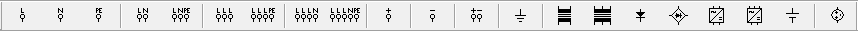
\includegraphics[width=\linewidth]{cam/cam3.png}
Fusibles, seccionadores

\includegraphics[width=\linewidth]{cam/cam4.png}
Automáticos, disyuntores
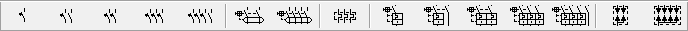
\includegraphics[width=\linewidth]{cam/cam5.png}
Contactores, interruptores
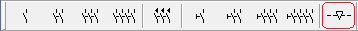
\includegraphics[width=\linewidth]{cam/cam6.png}
Motores

\includegraphics[width=\linewidth]{cam/cam7.png}
Potencia
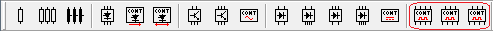
\includegraphics[width=\linewidth]{cam/cam8.png}
Contactos
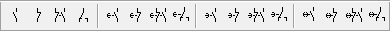
\includegraphics[width=\linewidth]{cam/cam9.png}
Accionamiento

\includegraphics[width=\linewidth]{cam/cam10.png}
Detectores
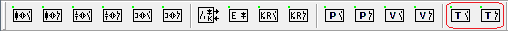
\includegraphics[width=\linewidth]{cam/cam11.png}
Bobinas, señalizaciones
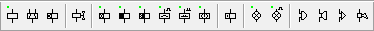
\includegraphics[width=\linewidth]{cam/cam12.png}
Relés electrónicos
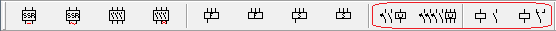
\includegraphics[width=\linewidth]{cam/cam13.png}
Lógica
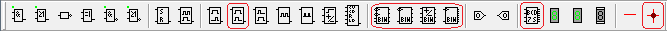
\includegraphics[width=\linewidth]{cam/cam14.png}
Ladder
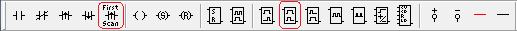
\includegraphics[width=\linewidth]{cam/cam15.png}
Grafcet

\includegraphics[width=\linewidth]{cam/cam16.png}
Entrada/Salida
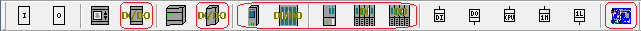
\includegraphics[width=\linewidth]{cam/cam17.png}
Electroneumática

\includegraphics[width=\linewidth]{cam/cam18.png}
Símbolos imagen 2D

\includegraphics[width=\linewidth]{cam/cam19.png}
Símbolos imagen 3D

\includegraphics[width=\linewidth]{cam/cam20.png}
Cables y conexiones
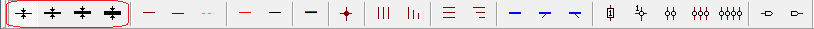
\includegraphics[width=\linewidth]{cam/cam21.png}
\end{center}
\begin{notation}
La clave del CADe Simu es 4962 y del PC Simu es 9966.
\end{notation}
\subsection{Simulaciones}
Para poder realizar circuitos en CADe Simu, necesitamos tener en cuenta los siguientes pasos:
\begin{enumerate}
\item Realizar el esquema insertando los componentes eléctricos.
\item Los distintos componentes siempre se tendrán que conectar a través del distinto cableado, NO se pueden conectar los distintos componentes de forma directa sin el cableado.
\item En un circuito eléctrico se tiene que partir siempre de una alimentación pudiendo ser de corriente continua o corriente alterna. La librería de alimentaciones permite seleccionar una gran variedad de símbolos de alimentación.
\item Durante la simulación se realiza una comprobación de la existencia tanto de cortocircuitos y de conexiones a masa. Si se produce uno de estos errores la simulación se para y se nos advierte con el correspondiente mensaje.
\item En un esquema los distintos símbolos de un mismo componente tienen que tener el mismo nombre y no se puede repetir con símbolos de otros componentes.
\end{enumerate}

\begin{example}[Arranque de motor trifásico con sistema de parada de emergencia]
Nos piden diseñar un arranque de motor trífasico con botones de Start y Stop, además que tenga un sistema de protección si el motor se sobre carga.\\
\textbf{Solución}\\
\textbf{Circuito de mando:}\\
Empezamos con dos relés térmicos: NA (normalmente abierto) y NC (normalmente cerrado). Estos van a actuar al mismo tiempo, por eso les ponemos el mismo nombre: \textit{-F2}. Con esta configuración podemos desviar la corriente de la rama principal, en la cual irá el circuito de arranque, de la rama de emergencia.
\begin{center}
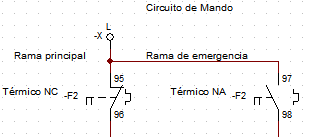
\includegraphics[width=0.5\linewidth]{cam/cam22.png}
\end{center}
En la \textbf{rama principal} pondremos un pulsador NC con el nombre \textit{-S1}. Colocamos un NC pues inicialmente la corriente debe fluir hacia debajo de este. Si accionamos el pulsador \textit{-S1}, este se abrirá y hará que el circuito por debajo de este deje de energizarse: Esto nos servirá como interruptor de apagado. Seguidamente pondremos en paralelo un pulsador NA con el nombre \textit{-S2} y un contacto NA con el nombre \textit{-KM1}. Este contacto se activará al pulsar \textit{-S2}. Lo sé, no tienen el mismo nombre pero haremos que funcione con una ``memoria''. La ``memoria'' va ser reemplazada por una bobina que se encuentra en serie del pulsador \textit{-S2}. Añadiremos un piloto señalizador verde que nos indique que el motor esta funcionando.
\begin{center}
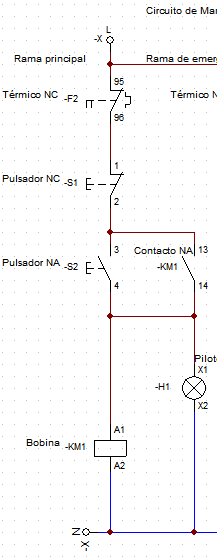
\includegraphics[width=0.3\linewidth]{cam/cam23.png}
\end{center}
Resumiendo hasta ahora: el térmico \textit{-F2} y el pulsador \textit{-S1} harán pasar la corriente hasta \textit{-S2}. Si este último se presiona, cargará la bobina y este a su vez mantendrá activado el contacto \textit{-KM1}, además se encenderá el piloto \textit{-H1}.\\
En la \textbf{rama de emergencia}, el térmico NA \textit{-F2} se cerrará cuando el térmico NC \textit{-F2} se abra, en otras palabras cuando exista una emergencia, la corriente se desviará completamente de la rama principal a la rama de emergencia. En esta rama pondremos solo un piloto rojo a manera de indicar que ha sucedido un problema: piloto rojo \textit{-H2}.\\
\textbf{Circuito de potencia}:
Poniendo de antemano la alimentación en fase correspondiente pondremos un contactor III con el nombre \textit{-KM1}. Cuando se active la bobina, este mantendrá el piloto \textit{-H1} activado y también el motor. Seguidamente pondremos un relé térmico \textit{-F2}. Esté será el encargado de activar los térmicos \textit{-F2} de emergencia. Finalmente colocamos el motor.
\begin{center}
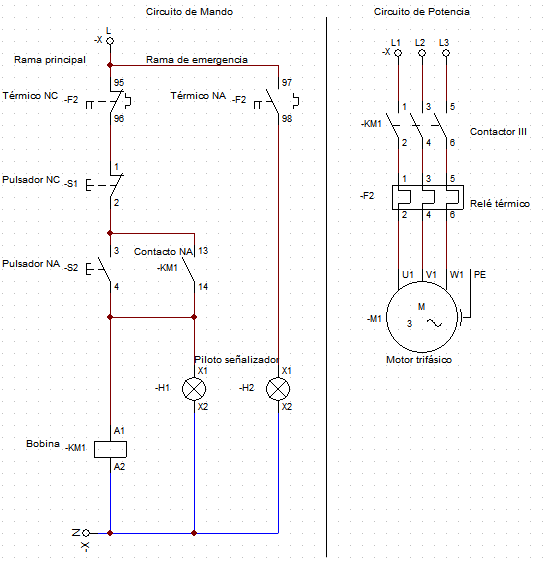
\includegraphics[width=0.6 \linewidth]{cam/cam24.png}
\end{center}
\end{example}
\begin{remark}
Recuerda, para alimentación Fase necesitas \textcolor{red}{cable fase} y alimentación Neutro necesitas \textcolor{blue}{cable neutro}.
\end{remark}
\begin{example}[Realizar dos fajas transportadoras con modo Manual y Automático]
Se requiere dos fajas transportadoras que funcionen de dos modos:
\begin{itemize}
\item \textbf{Manual}: Botón de encendido que empiece la marcha de las fajas y motor de detención para detener todo.
\item \textbf{Automático}: Si se detecta un objeto al inicio de la faja, que empiece a funcionar.
\end{itemize}
\textbf{Solución}:\\
\textbf{Circuito de Mando}:\\
Tomaremos parte del circuito del anterior ejemplo. Empecemos con el modo \textbf{manual}, habrá un botón para poder entrar a este modo al igual que con el modo automático. Al ser un ``menú'', tenemos que usar pulsadores NA (solo se activarán cuando nosotros lo presionemos), Cuando se presione este pulsador \textit{-S1}, vamos a guardar su estado usando la bobina \textit{-K5}, a su vez esta bobina \textit{-K5} mantendrá activo el contacto NA \textit{-K5}. Estamos usando también un contacto NC \textit{-K6} para apagar este modo manual. Más tarde veremos como lo usaremos:\\
\begin{center}
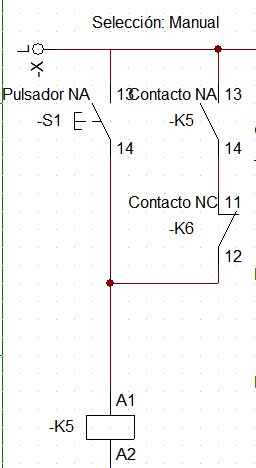
\includegraphics[width=0.4\linewidth]{cam/cam25.png}
\end{center}
Cuando la energía llegué a \textit{-K5} indica que el modo manual ha sido activado, es por esta razón que procedemos a activar los motores. Al igual que el ejemplo anterior, tendremos una rama (principal) de control y la otra de emergencia. Para este paso no vamos a explicar pues el mismo funcionamiento, la única diferencia es que tanto el rama de control como la de emergencia esta siendo activo solo si el contacto NA \textit{-K5} se cierra, y eso sucede cuando el seleccionamos modo manual. En este ejercicio el pulsador \textit{-S3} representa \textbf{stop} y el pulsador \textit{-S4} representa \textbf{start}:
\begin{center}
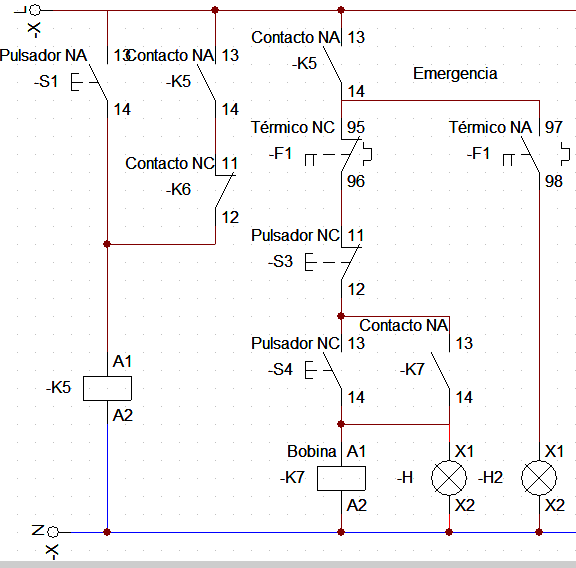
\includegraphics[width=0.4\linewidth]{cam/cam26.png}
\end{center}
Finalmente, la bobina \textit{-K7} encenderá los contactos NA \textit{-K7}, que a su vez energizarán las bobinas de los motores.
\begin{center}
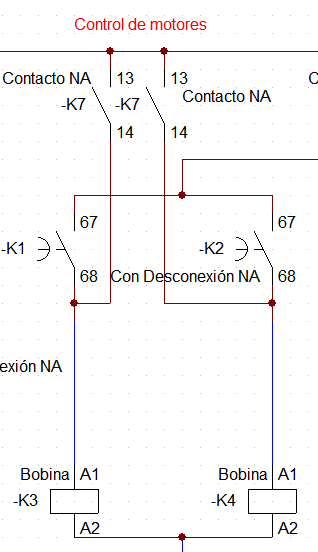
\includegraphics[width=0.4\linewidth]{cam/cam28.png}
\end{center}
\textbf{Modo Automático}\\
Para la selección de este modo es muy similar al anterior, nota que aquí estamos haciendo uso del contacto NC \textit{-K6}, este contacto nos ayuda a apagar el otro modo, es decir, si se selecciona el modo manual, el modo automático se apaga y viceversa.
\begin{center}
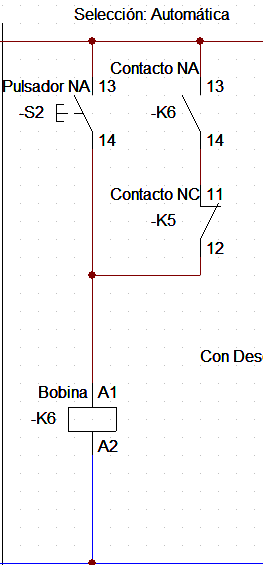
\includegraphics[width=0.2\linewidth]{cam/cam27.png}
\end{center}
Cuando se seleccione el modo auto, el contacto \textit{-K6} se encenderá ayudado por la bobina \textit{-K6}. Este contacto \textit{-K6} activará los detectores inductivos NA \textit{-B1} y \textit{-B2}. 
\begin{center}
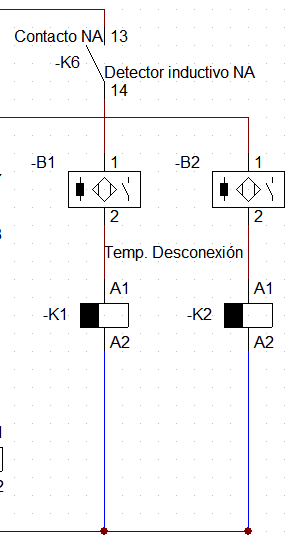
\includegraphics[width=0.35\linewidth]{cam/cam29.png}
\end{center}
Esto quiere decir que los detectores no dejarán pasar energía a no ser que detecten algo, es ahí cuando se cierran y se activarán los temporizadores, el temporizador a su vez cierra el contacto desconexión NA \textit{-K1} energizando la bobina del motor \textit{-K3}. 
\begin{center}
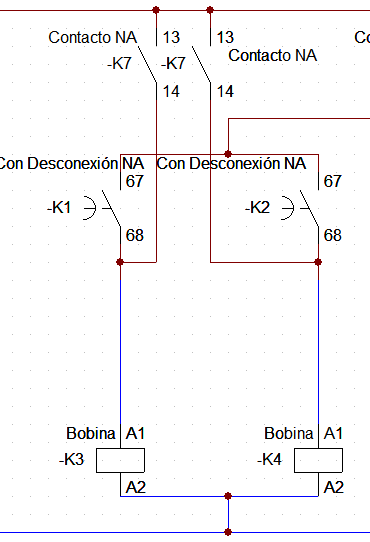
\includegraphics[width=0.3\linewidth]{cam/cam30.png}
\end{center}
\textit{-K1} estará encendido durante 3 seg (se configura en el temporizador de desconexión), pasado ese tiempo \textit{-K1} se desconecta apagando el motor. El proceso es exactamente lo mismo para el detector inductor \textit{-B2}.
La parte de los motores es la misma que el ejemplo anterior.\\
\begin{center}
Circuito en CADe Simu\\
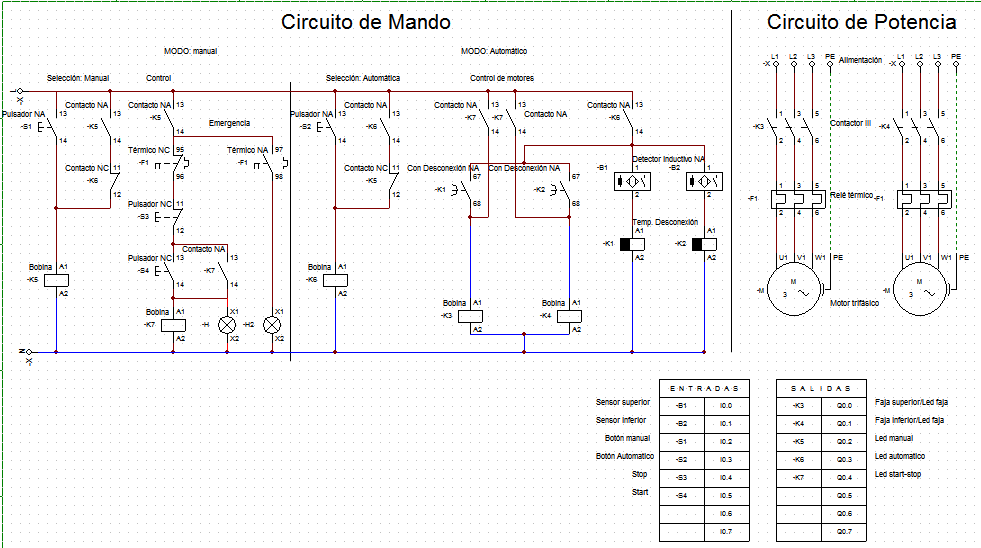
\includegraphics[width=0.85\linewidth]{cam/cam31.png}
\end{center}
\begin{center}
Simulación en PC Simu\\
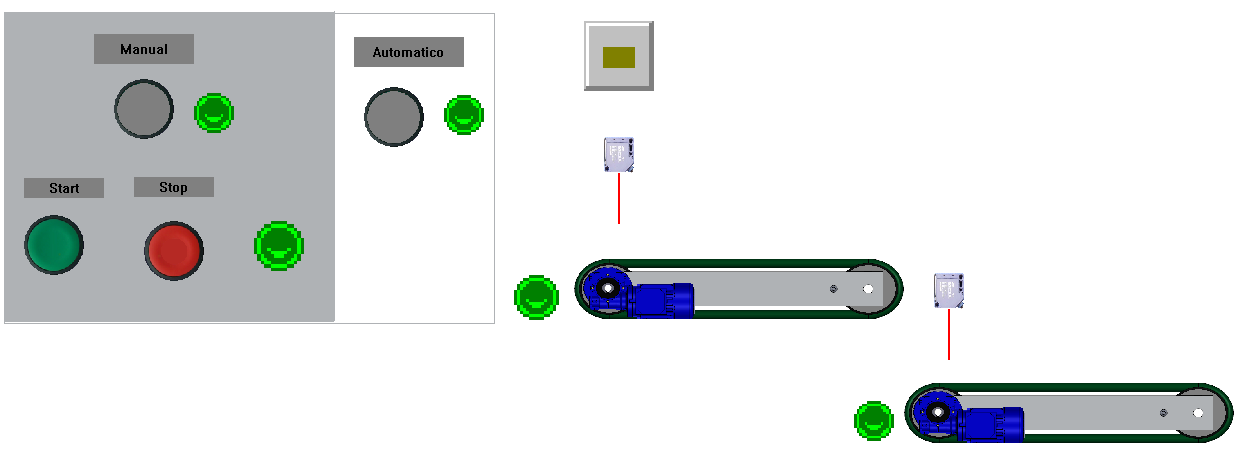
\includegraphics[width=0.8\linewidth]{cam/cam32.png}
\end{center}
\end{example}
\subsection{Ladder}\index{Ladder}
Ladder es escalera en inglés. El nombre por lo tanto recuerda que este lenguaje de programación se programa mediante símbolos gráficos y en diferentes segmentos. Como en las escaleras, en cada segmento (o escalón), programamos las diferentes sentencias de la lógica. Al lenguaje Ladder también se le conoce como diagrama de contactos, puesto que realmente programamos mediante contactos eléctricos que, unidos, terminan formando una sentencia lógica.\\
Ladder es uno de los diferentes lenguajes de programación para los controladores lógicos programables (PLCs) estandarizados con IEC 61131-3. En Ladder, la energía se desplaza de izquierda a derecha en lugar de arriba hacia abajo como en los esquemas eléctricos. En un circuito típico aparecen los contactos en la parte izquierda y una bobina en la parte derecha. La lógica de control que representa dicho circuito puede verse como una inferencia lógica que tiene como antecedente la lógica de los contactos y como concluyente la bobina.\\
Para programar un autómata con Ladder, además de estar familiarizado con las reglas de los circuitos de conmutación, (también denominada Lógica de Contactos), es necesario conocer cada uno de los elementos de que consta este lenguaje. A continuación se describen de modo general los más comunes (Fig. \ref{fig:basicos ladder})
\begin{itemize}
\item \textbf{Contacto normalmente abierto (E1)}: si la variable asociada E1 vale ‘0’, el contacto permanece abierto, y si vale ‘1’ se cierra.
\item \textbf{Contacto normalmente cerrado (E2)}: si la variable asociada E1 vale ‘1’, el contacto permanece abierto, y si vale ‘0’ se cierra.
\item \textbf{Salida, bobina o relé (S1)}: la variable asociada S1 tomará el valor de la variable (o combinación de variables) que esté a su entrada (punto de conexión del lado izquierdo). También se puede enclavar o desenclavar, indicándolo con una S o R como se indica en los casos de S2 y S3.
\end{itemize}
\begin{figure}[]
\centering
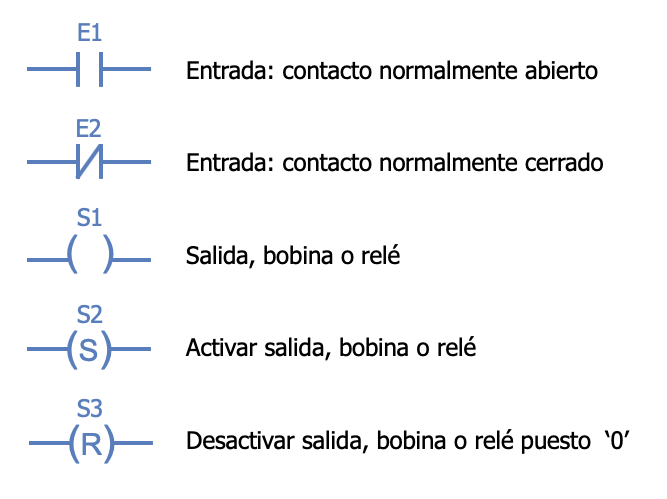
\includegraphics[width=0.5\linewidth]{CAM/cam33.png}
\caption{Elementos básicos de Ladder.}
\label{fig:basicos ladder}
\end{figure}
\begin{notation}
Una bobina normal puede verse como una asignación del valor lógico conectado a su izquierda. Por contra, una bobina de enclavamiento (S / R) se activa de la misma manera que la bobina anterior, pero retiene el valor (‘1’ / ‘0’) aunque el valor lógico conectado a su izquierda pase a ‘0’.
\end{notation}
\subsubsection{Compuertas lógicas}
Se pueden implementar funciones lógicas de forma sencilla. Por ejemplo, en la figura siguiente (Fig. \ref{fig:compuertas ladder}) se implementa un función AND y una OR.
\begin{figure}[H]
\centering
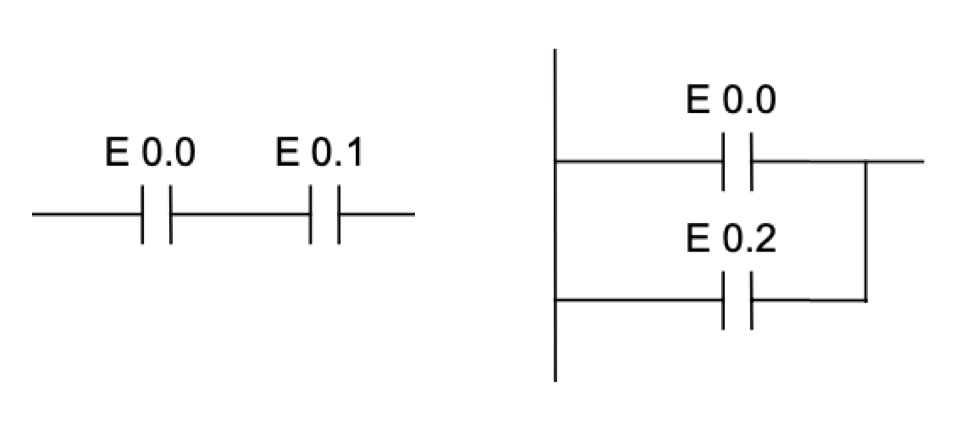
\includegraphics[width=0.5\linewidth]{CAM/cam34.png}
\caption{Elementos básicos de Ladder.}
\label{fig:compuertas ladder}
\end{figure}
A manera de explicar el lenguaje Ladder, vamos a arrancar un motor trifásico usando para ello un PLC LOGO\footnote{Disponible en la pestaña \textit{Entrada/Salida}>Módulo Lógico}; vamos a tener 3 botones de control: \textit{Start}, \textit{Stop} y uno auxiliar (puede ser de emergencia). En el PLC hacemos la conexión \textbf{Alimentación Fase} y \textbf{Alimentación Neutro}. Del positivo debemos tener las siguientes conexiones:
\begin{itemize}
\item P1: Conexión directa.
\item I1: Conexión por un pulsador NA.
\item I2: Conexión por un pulsador NA.
\item I3: Conexión por un pulsador NA.
\item Q1-1: Conexión directa.
\item Q2-1: Conexión directa.
\end{itemize}
El diagrama nos debe quedar como la figura \ref{fig:logo fase}\\
\begin{figure}[H]
\centering
\subfloat[Fase: parte superior]{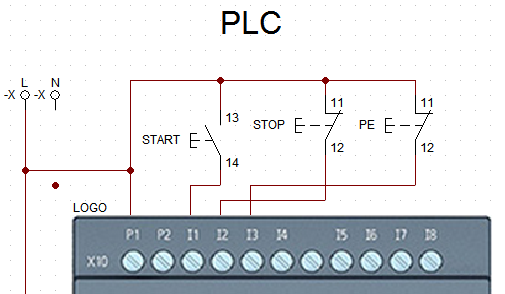
\includegraphics[width=0.5\linewidth]{CAM/cam35.png}}
\subfloat[Fase: parte inferior]{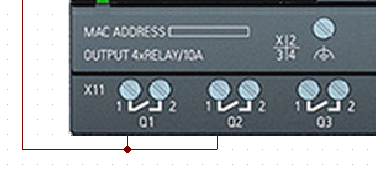
\includegraphics[width=0.5\linewidth]{CAM/cam36.png}}
\caption{Conexión fase.}
\label{fig:logo fase}
\end{figure}
Usando la alimentación neutra conectaremos la siguiente manera:
\begin{itemize}
\item P2: Conexión directa.
\item Q1-2: A la salida de una bobina, esta bobina debe tener el mismo nombres que los contactores III del motor.
\end{itemize}
El resultado del PLC debe ser como la figura \ref{fig:conexion plc}.
\begin{figure}[H]
\centering
\includegraphics[width=0.4\linewidth]{CAM/cam37.png}
\caption{Conexión PLC}
\label{fig:conexion plc}
\end{figure}
Recordando la Fig. \ref{fig:compuertas ladder}, más en específico usaremos la compuerta OR: es necesario que una de las entradas se active para que las energice lo demás. Empezamos colocando \textbf{Alimentación +} y \textbf{Alimentación -}. 
Configuramos la compuerta OR: la primera entrada/contacto que se cierre con el pulsador \textit{START} ó que se cierre con \textit{Q1} (Q1 va ser configurada luego como una retro-activación). Después de la compuerta OR vamos a tener contactos NC para que dejen pasar la energía inicialmente; estos serán \textit{PE} y \textit{STOP}. Al final de esta rama colocaremos una bobina \textit{Q1}, la que servirá como retroalimentación. (Fig. \ref{fig:ladder motor})
\begin{figure}[]
\centering
\includegraphics[width=\linewidth]{CAM/cam38.png}
\caption{Diagrama Ladder.}
\label{fig:ladder motor}
\end{figure}
\textbf{Funcionamiento}: Para que el motor pueda arrancar, necesitamos activar el pulsador \textit{START} para que la bobina \textit{Q1} se active y a su vez active el contacto \textit{Q1} para que se quede ``enganchado''. Esto se quedará enganchado hasta que los contactos NC se abran, esto solo pasará cuando los pulsadores \textit{STOP} y \textit{PE}se active, esto ocasionará que los contactos se abran y se interrumpa el circuito. El circuito final se gráfica en la figura \ref{fig:motor y logo}.
\begin{figure}[]
\centering
\includegraphics[width=\linewidth]{CAM/cam39.png}
\caption{Resultado final motor y PLC LOGO.}
\label{fig:motor y logo}
\end{figure}
\begin{remark}
Para PLC necesitas cable fase y cable neutro. Para ladder necesitas cable negativo y cable negativo. En PLC LOGO, P1 es puerto positivo y P2 es puerto negativo (en la parte superior: Dispositivos de entrada) y sirven para dar energía al PLC, por lo tanto hay que energizarlas. De igual manera con la parte inferior (Dispositivos de salida), se debe energizar positivamente las entradas 1 y los dispositivos deben estarn en las salidas 2 hacia negativo.
\end{remark}
\begin{example}[Diseñe una faja transportadora con el PLC LOGO, sensores y tenga apagado automático]
Para este proyecto se usaremos parte de encender un motor con ladder explicado anteriormente.\\
\textbf{PLC:}\\
Empezamos cambiando las entradas del PLC, esta vez no contaremos con pulsadores, al ser automático usaremos \textbf{sensores inductivos NA} (etiquetados con \textit{S1}, \textit{S2} y \textit{S3}) y un pulsador de detención \textit{STOP}.
\begin{center}
\includegraphics[width=0.6\linewidth]{cam/cam40.png}
\textbf{No te olvides de energizar el PLC.}
\end{center}
Por la parte inferior del PLC, conectaremos dos bobinas para cada motor, pues son dos motores, y en paralelo colocaremos pilotos. No es recomendable colocarlos en serie.
\begin{center}
\includegraphics[width=0.6\linewidth]{cam/cam41.png}
\end{center}
\textbf{Ladder}:\\
Para ladder vamos a usar el mismo mecanismo de accionamiento del motor visto antes, en este ejemplo usaremos dos ``memorias'' (\textit{M2} y \textit{M3}) NC.
\begin{center}
\includegraphics[width=0.6\linewidth]{cam/cam42.png}
\end{center}
¿Por qué las memorias? Necesitamos que tenga un apagado automático, es decir, cuando el sensor de inicio de carrera (\textit{S1} y \textit{S2}) de ambas fajas no detecte material y el sensor de fin carrera (\textit{S3}) detecte que es último material, debe pasar cierto tiempo y que se apague ambas bajas.\\
Esto lo haremos estableciendo el sensor \textit{S3} como normalmente abierto, y en la misma rama contactos NC de \textit{S1} y \textit{S2}, de esta manera cuando el sensor \textit{S3} detecte material y los sensores \textit{S1} y \textit{S2} NO detecten nada, activará el \textbf{temporizador de desconexión} \textit{-T1} (5 seg). El temporizador mantendrá la energía hasta pasado un tiempo, luego de ello se apagará. Si se activa \textit{M1} y el sensor \textit{S1} no detecta nada, esta última rama activará el \textbf{temporizador de conexión}, que pasado un tiempo (15 seg), activará la bobina \textit{M2}, si esta se activa apagará el motor 1. Lo mismo pasará con la última rama. Si no detectan nada en sus respectivos sensores y \textit{M1} ha sido activado confirmando que todos los sensores no detectan nada, procede a abrir los contactos \textit{M2} y \textit{M3} para apagar motores.
\begin{center}
\includegraphics[width=0.6\linewidth]{cam/cam43.png}
\end{center}
\end{example}
%----------------------------------------------------------------------------------------
%	NEW CHAPTER
%----------------------------------------------------------------------------------------
\part{Software de telecomunicaciones}
\chapterimage{chapter_head_SFT.pdf} % Chapter heading image

\chapter{Unidad I}
\section{XDR}
\section{RPC y RMI}
Llamada a procedimiento remoto o RPC es una técnica que utiliza  el modelo cliente-servidor para ejecutar  tareas es un proceso diferente como podría ser en una computadora remota. A veces solamente se le llama como a una función o subrutina remota.
\subsection*{RPC}
\begin{enumerate}
\item El cliente hace la llamada al procedimiento remoto mediante un mensaje a través de la red. Este se detiene ya que es un proceso síncrono (se envía el mensaje y se queda ``callado'' hasta que reciba una respuesta), es decir, necesita una respuesta del servidor para poder continua su ejecución.
\item El servidor recibe la petición y desempaqueta el mensaje para extraer la información necesaria para realizar la tarea.
\item El servidor ejecuta la tarea. Con esto nos referimos que como cliente, enviamos la información a otra computadora (servidor) para que nos haga el ``trabajo sucio''.
\item El servidor crea un mensaje de respuesta para el cliente que incluye el resultado de la tarea que este le pidió realizar.
\item El cliente recibe y desempaqueta el mensaje de respuesta del servidor. Continua con su ejecución normal.
\end{enumerate}
\begin{notation}
El servidor siempre va estar activo, su función es atender a varios clientes a la vez.
\end{notation}
\subsection*{STUB}
Es la pieza de código que le permite al servidor ejecutar la tarea que se le asignó. Se encarga de proveer la información necesaria para que el servidor convierta las direcciones de los parámetros que el cliente envió en direcciones de memoria válidos dentro del ambiente del servidor. Parte del código que se encarga de ``traducir'' los entornos de ambos, en otras palabras le explica al servidor (o viceversa) como debe interpretar los datos. A manera de ejemplo (solo para explicar): El cliente solicita una suma de 15+83 y manda 1853 al servidor; el servidor no sabrá que significa ese número, el \textit{stub} le dirá: ``El primer y tercer dígito es el primer sumando, además el segundo y cuarto es otro número'', 
con esto el servidor sabrá cuales son los datos. El servidor hace la suma (89) con los números y devuelve : 0089. Este resultado viaja al cliente, sin no antes pasar por el \textit{stub} que le dice: ``El resultado de la suma es el número conformado por el cuarto dígito y el tercer dígito''. En conclusión, el \textit{stub} acomoda los datos para que los datos puedan ser procesados por cada lado.
La representación de datos en cliente y servidor (\textit{big-endian} o \textit{little-endian}) podría discrepar, el \textit{stub} también provee la información necesaria para solucionar esta situación.\\
Una inconveniente con esto es que RPC es dependiente del lenguaje de programación que se utilice.
\begin{definition}[Socket]
Los \textbf{sockets} sirven para la comunicación entre programas (en una primera medida), y para comenzar una conexión debemos crear un \textit{socket}; para dicha conexión se necesita una dirección IP y un puerto para realizar la conexión.
\end{definition}
\subsection{RMI}
Es un paquete de JAVA que permite manejar objetos (y sus respectivos métodos) de manera remota, para utilizar los recursos de un servidor de manera transparente para el usuario local. Es el analogo a RMS pero en JAVA, de igual manera al \textit{stub} aquí se le conoce como \textbf{Skeletons}. La diferencia más notable es que RPC es una solicitud remota mientras que RMI genera una \textbf{máquina virtual}, cuando mando una solicitud al servidor, es simular como si se estuviera ejecutando en el mismo lugar (servidor).

\begin{enumerate}
\item El servidor proporciona un servicio RMI y el cliente llama a métodos del objeto ofrecido por el servicio.
\item El servicio RMI se debe registrar en un servicio de consulta para permitir a los clientes encontrar el servicio.
\item El J2SE incluye una aplicación llamada \textit{rmiregistry}, que lanza un proceso que permite registrar servicios RMI mediante un nombre. Este nombre identifica al servicio, esto se hace as´ı ya que en una maquina puede haber diferentes servicios.
\item Una vez que el servicio se ha registrado, el servidor esperará a que lleguen peticiones RMI desde
los clientes.
\item El cliente solicita el servicio mediante el nombre con el que fue registrado y obtiene una referencia al objeto remoto
\item El formato utilizado por RMI para representar una referencia al objeto remoto es el siguiente \url{rmi://hostname:puerto/nombreServicio}.
\item Una vez obtenida la referencia remota (ya sea mediante \textit{rmiregistry}, leyendo el URL de un archivo,...) los clientes pueden enviar mensajes como si se tratase de objetos ejecutándose en la misma máquina virtual.
\item Los detalles de red de las peticiones y las repuestas son transparentes para el desarrollador. Esto se consigue mediante el uso de \textit{stub} (a partir de la versión 1.2, ya que en la versión 1.1 se requería generar un skeleton).
\end{enumerate}
\begin{definition}[Skeleton]
La clase skeleton es una clase generada por RMI. Esta clase es la responsable de comunicarse con el \textit{stub} durante la comunicación RMI. Debe reconstruir los parámetros para formar los tipos primitivos y objetos, lo que es conocido como \textit{unmarshalling}.
\end{definition}
\begin{figure}[H]
\centering
\includegraphics[width=0.5\linewidth]{soft/soft1.png}
\caption{Arquitectura RMI}
\end{figure}
\section{CORBA}
CORBA (\textit{Common Object Request Broker Architectur}e) es una arquitectura abierta desarrollada por los miembros del OMG (\textit{Object Management Group}). Desde 1989 la misión del OMG ha sido la especificación de una arquitectura para un \textbf{bus software abierto}, o \textit{Object Request Broker} (ORB), sobre el que diversos componentes de objetos escritos por diferentes vendedores puedan interoperar a través de la red y de los sistemas operativos. Este estándar permite que los objetos CORBA realicen llamadas entre ellos sin conocer dónde residen los objetos a los que acceden o en qué lenguaje están implementados estos últimos. OMG define un lenguaje (\textit{Interface Definition Language}: IDL) usado para definir las interfaces de los objetos CORBA.
\subsubsection*{Características}:
\begin{itemize}
\item Los objetos CORBA pueden estar en cualquier sitio de la red
\item Los objetos CORBA pueden interoperar con objetos de otras plataformas
\item Los objetos CORBA pueden escribirse en cualquier lenguaje de programación para el que exista un "mapeado" (correspondencia) desde el OMG IDL a dicho lenguaje. Actualmente las correspondencias definidas incluyen Java, C++, C, Smalltalk, COBOL, y Ada).
\end{itemize}
La plataforma Java 2 SE 1.4 proporciona un ORB que cumple con la especificación de CORBA 2.3.1 y dos modelos de programación CORBA que utilizan el ORB CORBA para Java y el Internet InterORB Protocol (IIOP). Los dos modelos de programación son el \textit{modelo de programación RMI} (o RMI-IIOP), y el \textit{modelo de programación IDL} (o Java IDL).
\subsection{CORBA y EAI}
La integraciones de aplicaciones para empresa (EAI( se puede conseguir en cuatro fases:
\begin{itemize}
\item Nivel de datos
\item Nivel de interfaz de aplicación
\item Nivel de lógica de negocio.
\item Nivel de presentación
\end{itemize}
Normalmente se comienza con la integración a nivel de \textbf{datos}, y se continúa con la integración a nivel de \textbf{interfaz}, y posteriormente a nivel de \textbf{lógica del negocio}. En ambas fases (interfaz y negocio) el objetivo es el \textbf{reusar} la funcionalidad de las aplicaciones existentes.\\
El uso de aplicaciones existentes se conseguirá por:
\begin{itemize}
\item \textbf{Modificando el código fuente}: Debemos definir una o más \textbf{APIs} con las operaciones que necesitamos para acceder de forma externa, y conectar dichas operaciones con el código existente. CORBA es una tecnología adecuada para realizar esto. Para cada interfaz que queramos añadir a la aplicación deberemos definir un \textbf{nuevo objeto CORBA distribuido}, declararemos las operaciones de la interfaz y conectaremos cada operación con el código fuente de la aplicación existente.
\item \textbf{Mediante técnicas como screeen scraping o emulación de terminales}: Si el código fuente no está disponible, o si no disponemos de las herramientas necesarias para recompilar la apliación a partir del código fuente, o simplemente no queremos modificar el código fuente, podemos utilizar estas técnicas. \textbf{Sreen scraping} y emulación de terminales son apropiadas principalmente para aplicaciones basadas en caracteres, los wrappers simulan lo que teclea el cliente para realizar las funciones de las aplicaciones existentes y leer la pantalla para extraer los resultados. En este caso el uso de CORBA vuelve a resultar adecuado.
\end{itemize}
\subsection{Arquitectura CORBA}
CORBA consiste en la especificación de un modelo de objetos distribuido idependiente del lenguaje, sistema operativo y plataforma. La parte principal de CORBA es el ORB (Object Request Broker). ORB actúa como un bus de mensajes que transporta peticiones de invocación de operaciones y sus resultados sobre objetos CORBA, proporcionando la infraestructura de comunicación necesaria de forma que oculte todos los detalles de la comunicación entre objetos distribuidos. La \textbf{transparencia de localización} es la capacidad de acceder e invocar operaciones sobre un objeto CORBA sin necesidad de conocer dónde reside dicho objeto. La idea es que debería ser igualmente sencillo invocar una operación residente en una máquina remota que un método de un objeto en el mismo espacio de direcciones. La \textbf{transparencia de lenguaje de programación} proporciona la libertad de implementar la funcionalidad encapsulada un objeto usando el lenguaje más adecuado, bien por las habilidades de los programadores, la idoneidad del lenguaje para la tarea específica, o la elección de un ``tercer'' desarrollador que proporciona componentes ya creados (off-the-shelf components). La clave de este grado de libertad es un \textbf{lenguaje de definición de interfaces} que es neutral con respecto a la implementación, y que proporciona una separación entre la interfaz y su implementación. Dicho lenguaje se denomina \textbf{\textit{Interface Denifition Language}} (IDL), y se utiliza para definir las interfaces de los objetos, independientemente del lenguaje de programación en el que estén implementados. Es un lenguaje fuertemente declarativo, con un rico conjunto de tipos de datos para describir parámetros complejos. Una interfaz IDL actúa como un contrato entre los desarrolladores de objetos y los eventuales usuarios de dichos interfaces. También permite a los usuarios de CORBA compilar las definiciones de las interfaces en código oculto para la transmisión de peticiones de invocaciones a través de las redes y las arquitecturas de las máquinas sin necesitar ningún conocimiento sobre el protocolo de red utilizado, o incluso la localización del objeto involucrado.
\section{SOAP}
Protocolo de acceso simple a objetos o SOAP. 
que existen diversos tipos de web
services, uno de los que mayor impacto tiene es el tipo SOAP este tipo de servicio está basado en el intercambio de información mediante \textit{xml} y su principal protocolo de funcionamiento es el \textit{http}, sin embargo también puede ser enviado mediante otros protocolos como \textit{ftp}, \textit{pop3}, \textit{tcp} y colas de mensajería. \\
\textbf{Ventajas}:
\begin{itemize}
\item Permite agregar metadatos en sus atributos.
\item Permite definir espacios de nombres para evitar la ambigüedad en su descripción.
\item Cuenta con métodos de validación más potentes que los de \textit{json}.
\item Funciona bien en ambientes empresariales es decir comunicaciones de servidor a servidor.
\end{itemize}
Al usar SOAP con el protocolo \textit{http} el tipo de contenido del mensaje que utiliza este protocolo debe establecerse en \textit{xml} que requiere la agregación de una línea que contiene SOAPAction en que debe estar presente en la cabecera \textit{http}. Por último podemos decir que la entrada SOAPAction permite que los firewalls del destino identifiquen los mensajes SOAP.
%----------------------------------------------------------------------------------------
%	NEW CHAPTER
%----------------------------------------------------------------------------------------
\part{Microelectrónica en RF}
\chapterimage{chapter_head_MR.pdf} % Chapter heading image

\chapter{Unidad I}
\section{Ondas electromagnéticas}
Las ecuaciones de Maxwell, propuestas por primera vez por James Clerk Maxwell, reunen las leyes experimentales de la electricidad y el magnetismo. Estas ecuaciones desempeñan en el electromagnetismo un papel análogo, a las leyes de Newton en la Mecánica. Con estas ecuaciones Maxwell pudo demostrar la existencia de las ondas electromagnéticas. Estas ondas electromagnéticas son originadas por cargas eléctricas aceleradas y fueron producidas por primera vez en el laboratorio por Heinrich Hertz en 1887.
Maxwell mostró que la velocidad de las ondas electromagnéticas en el \textbf{espacio vacío} es:
\begin{equation}
c=\frac{1}{\sqrt{\mu_0\epsilon_0}}\approx 3\basedec{8} m/s
\label{eq:vel luz}
\end{equation}
En otro medio es:
\begin{equation}
v=\frac{c}{\sqrt{\epsilon_r}}
\label{eq:velocidad relativa}
\end{equation}
Los campos E y B de la OEM son \textbf{perpendiculares} entre sí. Ambos son perpendiculares a la dirección de propagación de la onda (onda transversal).Las magnitudes de E y B están en fase y se relacionan por la expresión:
\begin{displaymath}
E=c\cdot B
\end{displaymath}
\begin{figure}[H]
\centering
\includegraphics[width=0.8\linewidth]{mrf/mrf1.png}
\caption{Ondas electromagnéticas}
\end{figure}
\begin{figure}[H]
\centering
\includegraphics[width=0.9\linewidth]{mrf/mrf2.png}
\caption{Espectro electromagnético}
\end{figure}
Las ondas electromagnéticas se presentan cuando se aceleran las cargas eléctricas. Las antenas deben tener ciertas impedancias, en esto es importante el tamaño de las antenas par evitar ROE, es por eso el tamaño el tamaño de las antenas deben estar en resonancia con la longitud de onda. Para este curso, trabajaremos con frecuencias desde $\basedec{3}-\basedec{6}$Hz aproximadamente. Altas frecuencias ya estaríamos hablando de microondas.
\begin{figure}[H]
\centering
\includegraphics[width=0.9\linewidth]{mrf/mrf3.png}
\caption{Espectro electromagnético con ejemplos.}
\end{figure}
\subsection*{Infrarojos}
La radiación infrarroja (IR) es una radiación electromagnética cuya longitud de onda comprende desde los 760-780 nm, limitando con el color rojo en la zona visible del espectro, hasta los 10.000 o 15.000 nm (según autores), limitando con las microondas. 
\subsection*{Ultravioleta}
Se denomina radiación ultravioleta o radiación UV a la radiación electromagnética cuya longitud de onda está comprendida aproximadamente entre los 100 nm ($100\cdot\basedec{-9}$ m) y los 400 nm ($400\cdot\basedec{-9}$ m). Su nombre proviene del hecho de que su rango empieza desde longitudes de onda más cortas de lo que el ojo humano identifica como luz violeta, pero dicha luz o longitud de onda, es invisible al ojo humano al estar por encima del espectro visible. Esta radiación es parte integrante de los rayos solares y produce varios efectos en la salud al ser una radiación entre no-ionizante e ionizante.
\subsection*{Rayos X}
Los rayos X son ondas de energía extremadamente alta con longitudes de onda entre 0.03 y 3 nanómetros, no mucho más largas que un átomo. Los rayos X son emitidos por fuentes que producen temperaturas muy altas como la corona del sol, que es mucho más caliente que la superficie.
\subsection*{Rayos gamma}
Rayos gamma. Longitud de onda igual o menor a $\basedec{-17}$ m. Frecuencia igual o superior a $\basedec{25}$ Hz. La región de los rayos gamma del espectro electromagnético se solapa con la de los rayos X. La radiación gamma es producto principalmente de los núcleos inestables de materiales radiactivos artificiales y naturales. También son un componente de la llamada radiación cósmica, radiación que baña la Tierra procedente del espacio exterior. Son rayos muy penetrantes y producen daños serios si son absorbidos por tejidos vivos. En consecuencia, quienes trabajan cerca de este tipo de radiación peligrosa, deben estar protegidos con materiales de gran absorción, como gruesas capas de plomo.
\section{Distorsión}
Tengamos un sistema donde la respuesta ideal es \textit{x(t)}, en realidad no se obtendrá esa señal, por el contrario, obtendremos \textit{y(t)}, esta señal no es la ideal pues puede haberse visto alterada por distintos factores. Se define el error como:
\begin{equation}
e(t)=y(t)-x(t)
\end{equation}
Con esto en mente, podemos definir la distorsión como:
\begin{definition}[Distorsión]
Es cualquier cambio en una señal que altera su forma de onda básica (en el dominio del tiempo) o bien, altera la relación entre sus componentes espectrales (domino de la frecuencia). La distorsión puede ser del tipo \textbf{lineal} o del tipo \textbf{no lineal}. Relación de las potencia medias del error y de la señal.
\begin{equation}
D=\frac{\langle e^2(t)\rangle}{\langle y^2(t)\rangle}=\frac{P_e}{P_y}
\end{equation}
Donde:
\begin{itemize}
\item $e(t)$: Error.
\item $y(t)$: Señal obtenida.
\item $P_e$: Potencia del error. (W)
\item $P_y$: Potencia de la señal recibida. (W)
\end{itemize}
\end{definition}
La distorsión nace de los elementos reales: transmisor, línea de transmisión, antenas, etc. La distorsión no solo afecta la amplitud, puede afectar fase, información dada, etc.
\subsection{Distorsión lineal}\index{Distorsión lineal}
Una distorsión es lineal cuando la respuesta en frecuencia del circuito que trata a dicha
señal no es de una amplitud constante, o cuando se producen variaciones de fase en dicha señal.
En otras palabras, una distorsión lineal provoca el mismo porcentaje de error en una señal grande
que en una pequeña.\\
Existen distorsión de amplitud en la conversión de FM-AM por ejemplo. Ecos y reflexiones múltiples, los rebotes o propagación con trayectoria.\\
En un canal sin distorsión, supongamos que tenemos la siguiente señal:
\begin{displaymath}
y(t)=G\cdot x(t-\tau)
\end{displaymath}
Tenemos un desfase en $\tau$. Nuestra respuesta el lineal e invariante con el tiempo; en amplitud es contante con $\omega$ y la respuesta en fase es lineal con $\omega$.
\begin{figure}[H]
\centering
\includegraphics[width=.8\linewidth]{mrf/mrf5.png}
\caption{Canal de distorsión.}
\end{figure}
En una \textbf{distorsión de amplitud}, la respuesta espectral varía en amplitud con la frecuencia, la modulación PM/FM genera una modulación AM. 
\begin{figure}[H]
\centering
\includegraphics[width=.8\linewidth]{mrf/mrf6.png}
\caption{Distorsión en FM-AM.}
\end{figure}
Para \textbf{distorsión de fase}, 
\begin{figure}[H]
\centering
\includegraphics[width=.8\linewidth]{mrf/mrf7.png}
\caption{Distorsión de fase: retardo no uniforme.}
\end{figure}
\subsection*{Distorsión lineal por ecos}
\subsubsection*{Ecos y reflexiones múltiples}
En la actualidad existen \textit{n} portadoras de donde sea (artificiales y naturales), para un sistema OFDM, nuestra señal es dividida en pedazos pequeños o portadoras desfasadas, que hacen que reboten en distintos puntos antes de llegar al receptor. El objetivo es evitar que la toda la información se pierda por perdida de línea.
\subsubsection*{Distorsión por ecos}
Las señales que se retardan pueden sumarse a la fundamental, estos pueden ser causadas por ecos, es decir tienen la misma información pero están corridas en el tiempo, esto produce respuestas en amplitud y fase ondulada. Para resolver este problema usamos un ecualizador para cancelar ecos.
\begin{figure}[H]
\centering
\includegraphics[width=.8\linewidth]{mrf/mrf8.png}
\caption{Cancelar ecos: receptor Rake.}
\end{figure}
Si hay llegado múltiples portadoras, habrá un amplificador para ajustar la amplitud a la llegada, luego de ellos se les añadirá un retardo ajustable (aparte del retardo con el que llegó la señal) hasta que los retardos de las portadoras coincidan con un múltiplo del receptor principal. Finalmente resta la señal a la señal principal (Fundamentos del receptor Rake).
\begin{example}[Considere un sistema formado por un transmisor de TV analógica y una antena unidos por un cable coaxial, que consideramos sin pérdidas, de 150m de longitud y lleno de un dieléctrico de constante dieléctrica $\epsilon=2$. La señal de televisión está formada por una portadora de 600 MHz con una banda de modulación de 7.5 MHz. El coeficiente de reflexión a la salida del transmisor es de -10dB, y por un fallo en la conexión a la antena se produce una reflexión a su entrada de -5dB.]
\textbf{Determinando el retardo de la señal a lo largo del cable}:\\
Para el cable coaxial (que no es el vacío), el modo TEM, la velocidad de propagación usando la ecuación \ref{eq:velocidad relativa} es:
\begin{displaymath}
v=\frac{3\basedec{8}}{\sqrt{2}}=212\basedec{6}m/s
\end{displaymath}
Usando la ecuación del tiempo en función de la longitud:
\begin{displaymath}
\tau=\frac{150m}{212\basedec{6}m/s}=707.5ns
\end{displaymath}
Este retardo nos servirá solo si tenemos una medida con quien comparar, de lo contrario es imperceptible.
\textbf{¿Cuál será la amplitud de la señal reflejada en ambos extremos respecto de la señal directa?}\\
Aproximadamente, y si la reflexión es pequeña, el eco generado por reflexión tiene una relación de amplitud y fase en tensión con la señal directa dada por:
\begin{displaymath}
\frac{Eco}{Señal}\approx\Gamma_1\Gamma_2\exp(-2jkL)
\end{displaymath}
Pasando las unidades de decibelios a unidades lineales (recordando que son decibelios de voltaje) tenemos:
\begin{displaymath}
Eco\approx 0.1736 Señal
\end{displaymath}
La parte $\exp(-2jkL)$ viene del movimiento senoidal/cosenoidal y puede ser tomada como +1 y -1 pues son los máximos.\\
\textbf{Determine el rizado en amplitud y fase de la función de transferencia}\\
Si las reflexiones son pequeñas, y salvando un facto de fase, la función de transferencia puede aproximarse por:
\begin{displaymath}
H(\omega)\approx 1+\Gamma_1\Gamma_2\exp(-2jkL)=1+\Gamma_1\Gamma_2\exp(-2j\omega\tau)
\end{displaymath}
La fase de reflexión varía dentro de la banda $2(\omega_2-\omega_1)\tau=66.9 rad$ (más de diez vueltas), y, por tanto, los valores máximos y mínimos de amplitud y fase dentro de la banda serán:
\begin{align*}
|H(\omega)|_{máx}\approx 1+\Gamma_1\Gamma_2=1.18 \simeq 1.35dB\\
|H(\omega)|_{min}\approx 1-\Gamma_1\Gamma_2=0.83 \simeq -1.70dB\\
arg\left[\right]_{máx}\approx atan(\Gamma_1\Gamma_2)=0.176 rad \simeq 10.1°\\
arg\left[\right]_{min}\approx a-tan(\Gamma_1\Gamma_2)=-0.176 rad \simeq -10.1°
\end{align*}
\end{example}
\subsection{Distorsión no lineal}\index{Distorsión no lineal}
Esta distorsión es más difícil de tratar, tiene un comportamiento aleatorio, al no ser lineales las funciones de transferencia poseen valores cuadráticos.
\begin{figure}[H]
\centering
\includegraphics[width=0.8\linewidth]{mrf/mrf9.png}
\caption{Distorsión no lineal: Función de transferencia polinómica.}
\end{figure}
Vemos que el resultado es de una forma polinómica, y nosotros al querer de bajar de grado los polinomios usando identidades trigonométricas vamos a generar constantes, que se tratan como componentes en \textbf{continua}, estos pueden ser eliminados con condensadores. Tenemos saturación, componentes que hacen que la amplitud de nuestra señal se eleve considerablemente, estos consumirán energía y se controlan con atenuación pasiva .Por último tenemos \textbf{armónicos}, estos pueden consumen energía y consumen espectros de otras bandas que no se nos fueron asignadas, debemos aplicar filtros para controlarlos. Esto se llama \textbf{distorsión armónica}.
\begin{figure}[H]
\centering
\includegraphics[width=0.6\linewidth]{mrf/mrf10.png}
\caption{Ganancia y potencia de salida en un proceso de saturación.}
\end{figure}
Nota que se da un margen de 1 dB para poder calcular la potencia de saturación. Esta potencia a 1dB se llama \textbf{punto de compresión de 1dB}: Potenica a la salida en que la ganancia se ha reducido un decibelio.\\
Como lo visto, cuando se inyecta un tono sinusoidal puro en el modelo no lineal, la salida contiene varias componentes de diferentes frecuencias que toman las amplitudes siguientes:
Entrada:
\begin{displaymath}
v_1=A\cos(\omega_0t)
\end{displaymath}
Salida:
\begin{align*}
v_2&=k_1A\cos(\omega_0t)+k_2A^2\cos^2(\omega_0t)+k_3A^3\cos^2(\omega_0t)+\cdots\\
&=\frac{k_2A^2}{2}+\left(k_1+\frac{3k_3A^2}{4}\right)A\cos(\omega_0t)+\cdots
\end{align*}
Donde $P=\frac{(k_1A)^2}{2}$ es la potencia de salida en régimen lineal. El punto de compresión de 1 dB se obtiene para una ganancia de tensión que se ha reducido en 1 dB: $g_v=0.981k_1$. En ese punto, la potencia de salida viene dada por $P_{1dB}=0.794P$. Según el modelo polinómico se cumple entonces:
\begin{displaymath}
P_{1dB}=-0.058\frac{k_1^3}{K_3}
\end{displaymath}
En amplificadores muy lineales la relación es pequeña (0.3dB), mientras que en amplificadores poco lineales puede ser grande (2dB), siendo típicamente del orden de 1dB.\\
En el estudio de procesos no lineales en amplificadoes de potencia, es frecuente referir la potencia de salida a la de saturación. Puede entonces definirse un \textit{potencia de salida relativa a saturación} (OPBO):
\begin{equation}
OPBO (dB)=P_{sat}(dBm)- P_0(dBm)
\label{eq:opbo}
\end{equation}
\begin{example}[Un amplificador de potencia trabaja con una señal de RF cuya relación de potencia media a potencia pico es de 0.2. Si el nivel de saturación está 2dB por encima del punto de compresión de 1dB que es de 50dBm:]
\textbf{Determine la potencia máxima de salida para que nunca se sature:}\\
Si se asocia la máxima potencia de salida al punto de compresión de 1dB, la potencia media será 7dB menor que la potencia de pico (factor 0.2).
\begin{align*}
P_{med}&=P_{pico}\cdot 0.2\\
\frac{P_{pico}}{P_{med}}&=5\simeq 6.99 dB
\end{align*}
La potencia de pico a la salida corresponde al punto de compresión de 1 dB. En realidad hay que estimar 1dB más por efectos de la compresión de ganancia, de forma que la potencia media es:
\begin{displaymath}
P_{med}(dBm)=P_{pico}(dBm)-7=\underbrace{P_{1dB}+1}_{P_{pico}}-7=44dBm
\end{displaymath}
\textbf{Determine la OPBO}:\\
El nivel de salida realtivo a saturación se puede obtener como:
\begin{displaymath}
OPBO(dB)=\underbrace{P_{sat}(dBm)}_{P_{pico}+1dB}- P_{media}(dBm)=52dB-44dB=8dB
\end{displaymath}
\end{example}
\subsubsection{Armónicos}\index{Distorsión de armónicos}
La saturación provoca la aparación de armónicos de la señal de entrada, son cortes en las señales saturan la señal transportadora. Los armónicos se eliminan por filtrado. Se mide en porcentaje la tensión eficaz de armónico respecto a la tensión de salida o en dB de potencia.
\begin{definition}[Nivel de armónico de orden N]
Para calcular el nivel de un armónico de orden N ($P{AN}$) en un punto de potencia de salida ($P_0$) diferente del especificado, se puede hacer el siguiente cálculo:
\begin{equation}
P_{AN}=P_{AN0}\left(\frac{P_{out}}{P_{ref}}\right)^N
\label{eq:potencia del armonico}
\end{equation}
Donde:
\begin{itemize}
\item $P_{out}$: Potencia de salida. (W)
\item $P_{ref}$: Potenia de salida en un punto tomado como referencia para la medida del nivel del armónico. (W)
\item $P_{AN0}$: Potencia de referencia para un nivel de armónico. (W)
\end{itemize}
La ecuación \ref{eq:potencia del armonico} se puede expresar en dBm como:
\begin{equation}
P_{AN}(dBm)=P_{AN0}(dBm)+N(P_0(dBm)-P_{ref}(dBm))
\label{eq:potencia armonico dbm}
\end{equation}
\end{definition}
\begin{example}[Un amplificador de potencia lejos de la saturación genera un distorsión no lineal de forma que, al poner a la entrada una señal formada por un tono puro con una potencia de 10 dBm, a la salida produce una potencia n fundamental de 22 dBm y, medido en el analizador de espectros, se ha detectado un segundo armónico de -10 dBm y un tercer armónico de potencia igual a -18 dBm Determine La potencia de segundo y tercer armónico para una potencia de salida de 26 dBm]
La potencia de referenia en la medida de armónios es $P_{ref}=22 dBm$. De acuerdo con la ecuación \ref{eq:potencia armonico dbm}, hemos aumentado la potencia de salida en $P_0-P_{ref}=4dB$, lo que significa que el segundo armónico aumentará en 8 y el tercero en 12 dB:
\begin{align*}
P_{A2}(dBm)&=P_{A20}(dBm)+2(P_0(dBm)-P_{ref}(dBm))=-10+8=-2dBm\\
P_{A3}(dBm)&=P_{A30}(dBm)+3(P_0(dBm)-P_{ref}(dBm))=-18+12=-6dBm
\end{align*}
\includegraphics[width=0.8\linewidth]{mrf/mrf11.png}
\end{example}
\subsubsection{Intermodulación 3er orden: 2 tonos}
Ahora en vez de meter una sola señal (tono) a un amplificador no linean, vamos a meter dos tonos en diferente frecuencia:
\begin{figure}[H]
\centering
\includegraphics[width=0.8\linewidth]{mrf/mrf12.png}
\caption{Amplificador no lineal a 2 tonos.}
\end{figure}
Igualmente debemos ``bajar'' los exponentes a orden uno, aunque los términos aumentarán. La salida en frecuencia se vería así:
\begin{figure}[H]
\centering
\includegraphics[width=0.8\linewidth]{mrf/mrf13.png}
\caption{Intermodulación de tercer orden con dos tonos.}
\end{figure}
Nota que las combinaciones de frecuencias están a lo largo del dominio de frecuencia debido a la función de transferencia no lineal. A pesar de dos tonos, la amplificación esta generando 3 tonos.
\begin{figure}[H]
\centering
\includegraphics[width=0.8\linewidth]{mrf/mrf14.png}
\caption{Intermodulación de tercer orden con dos tonos: potencia.}
\end{figure}
La potencia asociada a los productos de intermodulación se define como:
\begin{equation}
I_3=CP_0^3
\end{equation}
Para potencia total de las señales de entrada ($P_{out}$) ubicado en el punto de intersección de tercer orden ($P_{out}=P\cdot I_3$):
\begin{align*}
&P_{out}=I_3=PI_3 &C=\frac{1}{P\cdot I_3^2}
\end{align*}
En función del punto de interseción ($PI_3$) y de la potencia de salida puede obtenerse la potencia de las componentes de intermodulación o su relación con la potencia de salida como:
\begin{equation}
I_3=P_{out}\left(\frac{P_{out}}{PI_3}\right)^2 \Rightarrow \frac{P_{out}}{I_3}=\left(\frac{PI_3}{P_{out}}\right)^2
\end{equation}
Donde $P_0$ es la potencia de salida en señal (las dos componentes), $PI_3$ es la potencia de slida en el punto de cruce e $I_3$ es la potencia total en los productos de intermodulación (las dos componentes).\\
Es frecuente trabajar con las potencia en unidades logarítmicas (dBm) o con las relaciones de potencias en dB, lo que aplicado a las expresiones anteriores queda como:
\begin{align}
I_3(dBm)&=3\cdot P_{out}(dBm)-2\cdot PI_3(dBm)\\
\left(\frac{P_0}{I_3}\right)(dB)&=2\cdot PI_3(dBm)-2\cdot P_{out}(dBm)
\end{align}
%ejercico diapo 29-distorsion
\section{Circuitos resonantes}
Un circuito resonante es una combinación de elementos sensibles a la frecuencia, conectados para obtener una respuesta selectora de frecuencia.
\subsection*{Circuito resonante en paralelo}
\begin{figure}[H]
\centering
\includegraphics[width=0.5\linewidth]{mrf/mrf16.png}
\caption{Circuito resonante en paralelo.}
\end{figure}
\begin{equation}
Y(\iu\omega)=G+\iu\omega C+\frac{1}{\iu\omega L}
\end{equation}
En paralelo, al buscar una igualdad entre la reactancia capacitiva y la inductiva, estos no entrarán en corto circuito, sino entrarán en circuito abierto. De este modo, la admitancia será tan solo la conductancia:
\begin{displaymath}
Y(\iu\omega_0)=G
\end{displaymath}
\begin{notation}
En serie, la impedancia en los elementos L y C tiende a 0, mientras que en paralelo tiende a infinito cuando el circuito esta en resonancia (funcionando con frecuencia de resonancia).
\end{notation}
Cuando se logra una impedancia o admitancia puramente real es cuando se trabaja en la \textbf{frecuencia de resonancia}, cuando se logra eso se dice que el circuito mismo está en \textbf{resonancia}. En la resonancia, el voltaje y la corriente están en \textbf{fase} y, por consiguiente, el \textbf{ángulo de fase es cero} y el \textbf{factor de potencia es unitario}.\\
En el caso en \textbf{serie}, en la resonancia, la \textbf{impedancia} es un \textbf{mínimo} y, por consiguiente, la \textbf{corriente es máxima} para un voltaje dado.
\begin{notation}
A bajas frecuencias, la impedancia del circuito en serie está dominado por el término capacitivo y la admitancia del circuito en paralelo está dominada por el término inductivo.\\
A altas frecuencias, la impedancia del circuito en serie está dominado por el término inductivo y la admitancia del circuito en paralelo está dominada por el término capacitivo.
\end{notation}
\begin{figure}[H]
\centering
\includegraphics[width=0.5\linewidth]{mrf/mrf17.png}
\caption{Gráficas del comportamiento en la frecuecnia de resonancia para serie y paralelo.}
\end{figure}
\begin{definition}[Función de transferencia en paralelo]
Realizando una asociación de admitancias en paralelo para hallar la función de transferencia sobre una fuente de corriente se obtiene:
\begin{equation}
H=\frac{1}{1+\iu\left(\omega\cdot C-\frac{1}{\omega\cdot L}\right)R}
\label{eq:funcion transferencia paralelo}
\end{equation}
\begin{definition}[Frecuencia de resonancia]
\begin{equation}
f_r=\frac{1}{2\pi\sqrt{L\cdot C}}
\label{eq:frec resonancia}
\end{equation}
Donde:
\begin{itemize}
\item $f_r$: Frecuencia de resonancia. (Hz)
\item \textbf{L}: Inductancia. (H)
\item \textbf{C}: Capacitancia. (F)
\end{itemize}
\end{definition}
\end{definition}
\begin{definition}[Factor de calidad-paralelo]
En esencia \textit{Q} es una medida de la capacidad de almacenamiento de energía de un circuito en relación con su capacidad de disipación de energía.
\begin{equation}
Q=\omega_r\cdot C\cdot R=\frac{R}{\omega_r\cdot L}=R\sqrt{\frac{C}{L}}
\label{eq:factor calidad paralelo}
\end{equation}
Donde:
\begin{itemize}
\item $\omega_r$: Frecuencia de resonancia. (rad/s)
\item \textbf{C}: Capacitancia. (F)
\item \textbf{R}: Resistancia. ($\Omega$)
\item \textbf{L}: Inductancia. (H)
\end{itemize}
\end{definition}
\begin{remark}
Cuando esta en resonancia, la función de transferencia debe ser igual a la unidad.
\end{remark}
Con el factor de calidad se puede llegar a una expresión para la función de transferencia expresada en la ecuación \ref{eq:funcion transferencia paralelo} :
\begin{equation}
H=\frac{1}{1+\iu Q\left(\frac{\omega}{\omega_0}-\frac{\omega_0}{\omega}\right)}
\end{equation}
Donde su magnitud y fase están dadas por:
\begin{align}
|H|&=\frac{1}{\left[+Q^2\left(\frac{\omega}{\omega_0}-\frac{\omega_0}{\omega}\right)^2\right]^{\frac{1}{2}}}\\
\phi&=-\tan^-1Q\left(\frac{\omega}{\omega_0}-\frac{\omega_0}{\omega}\right)
\end{align}
A ciertas frecuencias se obtiene los siguientes valores:
\begin{table}[H]
\centering
\begin{tabular}{|c|c|c|c|c|c|}
\hline
$\omega$ & 0   & $\omega_1$           & $\omega_0$ & $\omega_2$            & $\infty$ \\ \hline
|H|      & 0   & $\frac{1}{\sqrt{2}}$ & 1          & $-\frac{1}{\sqrt{2}}$ & 0        \\ \hline
$\phi$   & 90° & 45°                  & 0°         & -45°                  & -90°     \\ \hline
\end{tabular}
\caption{Valores importantes para el módulo y fase de H.}
\end{table}
Notamos que tenemos dos frecuecias: $\omega_1$ y $\omega_2$, que corresponden a $H=\frac{1}{\sqrt{2}}$. Examinando la ecuación de la magnitud H, se observa que $H=\frac{1}{\sqrt{2}}$ se presenta cuando:
\begin{equation}
Q^2\left(\frac{\omega}{\omega_r}-\frac{\omega_r}{\omega}\right)^2=1
\label{eq:h resonancia}
\end{equation}
La ecuación \ref{eq:h resonancia} se puede reordenar en forma de una ecuación de cuarto grado, en función de $\omega$. Despejando los valores de interés, se obtiene:
\begin{definition}[Frecuencias de media potencia]
Estos parámetros indican desde que frecuencias hasta que frecuencias opera nuestro circuito, en otras palabras limita el ancho de banda:
\begin{align}
\omega_1&=\omega_0\sqrt{1+\parentesis{\frac{1}{2Q}}^2}-\frac{\omega_r}{2Q}\\
\omega_2&=\omega_0\sqrt{1+\parentesis{\frac{1}{2Q}}^2}+\frac{\omega_r}{2Q}
\label{eq:limites de banda}
\end{align}
\end{definition}

\begin{definition}[Ancho de banda]
El ancho de banda (WB) del circuito se define como el intervalo que se encuentra entre las dos frecuencias donde la magnitud de la ganancia es $\frac{1}{\sqrt{2}}$ (-3dB). El ancho de banda de un circuito selectivo en frecuencia es el intervalo entre las frecuencias donde la magnitud de la ganancia cae a $\frac{1}{\sqrt{2}}$ veces el valor máximo.
\begin{equation}
WB=\omega_2-\omega_1=\frac{\omega_r}{Q}
\label{eq:ancho de banda resonancia}
\end{equation}
Donde:
\begin{itemize}
\item \textbf{WB}: Ancho de banda. (rad/s)
\item $\omega_2$: Frecuencia superior en -3dB. (rad/s)
\item $\omega_1$: Frecuencia inferior en -3dB. (rad/s)
\item $\omega_r$: Frecuencia de resonancia. (rad/s)
\item \textbf{\textit{Q}}: Factor de calidad.
\end{itemize}
\end{definition}
La ecuación \ref{eq:ancho de banda resonancia} ilustra que el ancho de banda es inversamente proporcional a \textit{Q}. Por tanto, la selectividad de frecuencia del circuito esta determinada por el valor de \textit{Q}. Un circuito de \textit{Q} alta tiene un ancho de banda pequeño y, por consiguiente, el circuito es muy selectivo.
\begin{figure}[H]
\centering
\includegraphics[width=0.5\linewidth]{mrf/mrf18.png}
\caption{Cuanto más alta \textit{Q}, tanto más pequeño el ancho de banda.}
\end{figure}
Cuando Q>10, las expresiones \ref{eq:limites de banda} se reducen a:
\begin{align}
\omega_1&\cong\omega_r-\frac{WB}{2}\\
\omega_2&\cong\omega_r+\frac{WB}{2}
\end{align}
Cuando Q>10, la curva de magnitud tiene una simetría aritmética aproximada entorno $\omega_r$. Independientemente de Q, la respuesta es simétrica en una escala logarítmica de frecuencia.
\begin{remark}
Si la banda de frecuencia que se va a seleccionar o a rechazar es estrecha, el \textit{Q} del circuito resonante debe ser alto. Si la banda de frecuencias es amplia, el \textit{Q} debe ser bajo.
\end{remark}
Para pequeñas desviaciones de frecuencias con respecto a $\omega_0$, \textit{Q} es relativamente alta y definimos $\delta$ como:
\begin{displaymath}
\delta=\frac{\omega-\omega_r}{\omega_r}=\frac{\omega}{\omega_r}-1
\end{displaymath}
donde $\delta$ representa la cantidad propocional por la que la frecuencia se desvía de $\omega_r$, entonces podemos escribir el siguiente factor en términod de $\delta$:
\begin{displaymath}
\frac{\omega}{\omega_r}-\frac{\omega_r}{\omega}=\parentesis{\delta+1}+\parentesis{\frac{1}{\delta+1}}=\frac{\parentesis{\delta+1}^2-1}{\delta+1}=\frac{\delta^2+2\delta}{\delta+1}
\end{displaymath}
Usando $\delta\ll 1$ para pequeñas desviaciones de $\omega_r$:
\begin{displaymath}
\frac{\omega}{\omega_r}-\frac{\omega_r}{\omega}\cong 2\delta
\end{displaymath}
Entonces H es:
\begin{equation}
H=\frac{1}{1+\iu 2Q\delta}
\end{equation}
Que es una aproximación valida siempre que $\delta\ll 1$.
\subsection*{Circuito resonante en serie}
\begin{figure}[H]
\centering
\includegraphics[width=0.5\linewidth]{mrf/mrf15.png}
\caption{Circuito resonante en serie.}
\end{figure}
Para un circuito RLC en serie, la \textbf{impedancia de entrada} se define:
\begin{equation}
Z(\iu\omega)=R+\iu\omega L+\frac{1}{\iu\omega C}
\end{equation}
Vemos que las reactancias inductivas y capacitivas se mueven, independientemente de sus valores L y C, con la frecuencia $\omega$, lo que se busca es que las reactancias se anulen para que nos quede la impedancia como un elemento netamente resistivo:
\begin{displaymath}
Z(\iu\omega_0)=R
\end{displaymath}
\begin{notation}
Que las reactancias se anulen significa que esos elementos funcionarán como un corto circuito.
\end{notation}
\begin{definition}[Función de transferencia en serie]
La función de transferencia para un circuito en serie esta dada por:
\begin{equation}
H=\frac{1}{1+\iu\parentesis{\frac{\omega\cdot L}{R}-\frac{1}{\omega CR}}}
\label{eq:funcion transferencia serie}
\end{equation}
\end{definition}
\begin{definition}[Factor de calidad-serie]
\begin{equation}
Q=\frac{\omega_r L}{R}=\frac{1}{\omega_rCR}=\frac{1}{R}\sqrt{\frac{L}{C}}
\label{eq:factor calidad serie}
\end{equation}
Donde:
\begin{itemize}
\item $\omega_r$: Frecuencia de resonancia. (rad/s)
\item \textbf{C}: Capacitancia. (F)
\item \textbf{R}: Resistancia. ($\Omega$)
\item \textbf{L}: Inductancia. (H)
\end{itemize}
\end{definition}
Con el factor de calidad se puede definir la ecuación \ref{eq:funcion transferencia serie} como:
\begin{equation}
H=\frac{1}{1+\iu Q\parentesis{\frac{\omega}{\omega_0}-\frac{\omega_0}{\omega}}}
\end{equation}
\begin{figure}[H]
\centering
\includegraphics[width=0.8\linewidth]{mrf/mrf19.png}
\caption{Resumen de osciladores: $\omega_0$ es la frecuencia de resonancia $\omega_r$}
\end{figure}
\section{Osciladores}
\subsection{Sistemas retroalimentados}
\begin{figure}[H]
\centering
\includegraphics[width=0.8\linewidth]{mrf/mrf20.png}
\caption{Sistemas retroalimentados.}
\end{figure}
De esta figura se desprenden dos ecuaciones que caracterizan a la función de transferencia:\\
\textbf{Lazo abierto: ganancia}
\begin{equation}
G(s)=\frac{x_s(S)}{x_{er}(s)}
\end{equation}
\textbf{Lazo cerrado: ganancia retroalimentada}:
\begin{equation}
\frac{x_s(s)}{x_e(s)}=\frac{G(s)}{1+G(s)\cdot H(s)}
\end{equation}
\begin{notation}
Si la retroalimentación es negativa, en la ecuación de lazo cerrado es positiva; igualmente si es positiva la retroalimentación, la ecuación es negativa.
\end{notation}
Algunos casos particulares que tenemos son:
\begin{itemize}
\item Realimentación negativa:
\begin{displaymath}
|1+G(s)\cdot H(s)|>1
\end{displaymath}
\item Alta ganancia de lazo: Cuando la ganancia es muy grande
\begin{displaymath}
\frac{x_s(s)}{x_e(s)}=\frac{1}{H(s)}
\end{displaymath}
\item Realimentación positiva:
\begin{displaymath}
|1+G(s)\cdot H(s)|<1
\end{displaymath}
\item Oscilación
\begin{displaymath}
|1+G(s)\cdot H(s)|=0
\end{displaymath}
La \textbf{oscilación} es indeseada en servosistemas y deseada en osciladores.
\end{itemize}
\subsection*{Caso de oscilación}
Si tenemos en cuenta la condición de oscilación, entonces se tendrá $x_s(s)/x_e(s)\rightarrow\infty$. Por lo tanto se genera una señal de salida ($x_s$) aunque no haya entrada ($x_e$)
\begin{figure}[H]
\centering
\includegraphics[width=0.6\linewidth]{mrf/mrf21.png}
\caption{Inversión de la red de retroalimentación}
\end{figure}
Cuando se esta oscilando, se tiene:
\begin{displaymath}
|G(s)\cdot H(s)|=1
\end{displaymath}
\begin{displaymath}
\fase{ }{G(s)\cdot H(s)}=180^{\circ}
\end{displaymath}
En oscilación:
\begin{displaymath}
|G(\iu\omega_r)\cdot H(\iu\omega_r)|=1
\end{displaymath}
\begin{displaymath}
\fase{ }{G(\iu\omega_r)\cdot H(\iu\omega_r)}=180°
\end{displaymath}
Graficando la oscilación en la figura \ref{fig:oscilacion}, nota como la señal sale en fase de la planta, en la salida llega la onda amplificada mientras que en la red de retroalimentación se atenúa  la señal un poco pero esta totalmente desfasada. Por mejor del bloque inversor esta se acoplada nuevamente a la onda. Con esto nos aseguramos que la oscilación ha comenzado.
\begin{wrapfigure}{r}{0.5\textwidth}%tamaño del campo asignado
  \begin{center}
    \includegraphics[width=0.45\textwidth]{mrf/mrf22.png}%tamaño del la imgen dentro del campo
  \end{center}
  \caption{Condición de oscilación.}
  \label{fig:oscilacion}
\end{wrapfigure}
\subsubsection{Condición de oscilación}\index{Condición de oscilación}
\textbf{¿Qué tiene que suceder para que comience la oscilación?}\\
Los circuitos osciladores son un tanto especiales, necesitamos para arrancar una señal de entrada que sirva como una señal de arranque ($x_e$) (Fig. \ref{fig:condi osci}).
\begin{figure}[]
\centering
\includegraphics[width=0.6\linewidth]{mrf/mrf23.png}
\caption{Condición de oscilación}
\label{fig:condi osci}
\end{figure}
Cuando el sistema termine de arrancar, cerramos el switch y podemos quitar la señal de entrada. Hay que asegurarnos que $|G\parentesis{\iu\omega_{osc}}\cdot H\parentesis{\iu\omega_{osc}}|>1$, cuando el desfase es 180$^{\circ}$, entonces podemos hacer que la salida del
lazo de realimentación haga las funciones de la magnitud de entrada.
\begin{wrapfigure}{l}{0.55\textwidth}
  \begin{center}
    \includegraphics[width=0.53\textwidth]{mrf/mrf24.png}
  \end{center}
  \caption{Oscilación.}
  \label{fig:oscilacion 1}
\end{wrapfigure}
En la figura \ref{fig:oscilacion 1} el sistema ya esta arrancando, pero no termina ahí, ahora debe calibrarse para que pueda auto-arrancar por si solo.\\\textbf{Momento de oscilación}
\begin{figure}[H]
\centering
\includegraphics[width=0.6\linewidth]{mrf/mrf25.png}
\caption{Transición a estable.}
\end{figure}
\begin{notation}
$G_{pm}(s)$ significa función de transferencia de pequeña magnitud. $G_{gm}(s)$: función de transferencia de gran magnitud.
\end{notation}
\subsubsection*{Criterio de Nyquist}
Para que \textbf{empiece} la oscilación:
\begin{itemize}
\item Tiene que existir una $\omega_{osc}$ a la que se cumpla:
\begin{displaymath}
\fase{}{G(\iu\omega_{osc})\cdot H(\iu\omega_{osc})}=180^{\circ}
\end{displaymath}
\item A esa $\omega_{osc}$ tiene que cumplirse:
\begin{displaymath}
|G(\iu\omega_{osc})\cdot H(\iu\omega_{osc})|>1
\end{displaymath}
\end{itemize}
Cuando se \textbf{estabiliza} la oscilación:
\begin{itemize}
\item Disminuye la ganancia
\begin{displaymath}
G(\iu\omega_{osc})
\end{displaymath}
hasta que
\begin{displaymath}
|G(\iu\omega_{osc})\cdot H(\iu\omega_{osc})|=1
\end{displaymath}
cuando
\begin{displaymath}
\fase{}{G(\iu\omega_{osc})\cdot H(\iu\omega_{osc})}=180^{\circ}
\end{displaymath}
\end{itemize}
\subsubsection*{Diagramas de Bode}
Observa la linea punteada, de la figura \ref{fig:cuando oscila}, debe ser corregida pues tanto la fase como la magnitud deben coincidir en la misma frecuencia a 0dB (o $|G(\iu\omega_{osc})\cdot H(\iu\omega_{osc})|$)
\begin{figure}[]
\centering
\subfloat[Cuando ya oscila.]{\includegraphics[width=0.25\linewidth]{mrf/mrf26.png}\label{fig:cuando oscila}}
\subfloat[Para que no oscile.]{\includegraphics[width=0.25\linewidth]{mrf/mrf27.png}}
\caption{Condición de oscilación}
\end{figure}
\begin{figure}[H]
\centering
\includegraphics[width=0.7\linewidth]{mrf/mrf28.png}
\caption{Resumen de arranque de osciladores.}
\end{figure}
%Osciladores hartley
\subsection{Osciladores de frecuencia muy constante}
\subsubsection*{Cristales osciladores}
Es un cristal de cuarzo (u otro material piezoeléctrico) que consta de una placa de cuarzo en medio de dos contactos metálicos, encapsulados. Se aplica voltaje en sus terminales para que vibren de manera tan exacta que es muy precisa.
\begin{wrapfigure}{r}{0.5\textwidth}
  \begin{center}
    \includegraphics[width=0.48\textwidth]{mrf/mrf29.png}
  \end{center}
  \caption{Símbolo cristal oscilador}
\end{wrapfigure}

\begin{wrapfigure}{l}{0.5\textwidth}
  \begin{center}
    \includegraphics[width=0.48\textwidth]{mrf/mrf30.png}
  \end{center}
  \caption{Cristal oscilador}
\end{wrapfigure}
\begin{figure}[]
\centering
\includegraphics[width=0.6\linewidth]{mrf/mrf31.png}
\caption{Circuito equivalente de un cristal de cuarzo.}
\end{figure}
%----------------------------------------------------------------------------------------
%	ANEXOS
%----------------------------------------------------------------------------------------
\part{Anexos}
%---------------------------------------------------------------
% 		ENDING
%---------------------------------------------------------------
\stopcontents[part] % Manually stop the 'part' table of contents here so the previous Part page table of contents doesn't list the following chapters
\section{Constantes universales}
\begin{itemize}
\item $\mu_0$: Permeabilidad en el vacío.
\begin{displaymath}
\mu_0=1.2566\cdot\basedec{-6} N/A^2
\end{displaymath}
\item $\epsilon_0$: Permitividad en el vacío:
\begin{displaymath}
\epsilon_0=8.854\cdot\basedec{-12} F/m
\end{displaymath}
\end{itemize}
\section{Voltajes}

%----------------------------------------------------------------------------------------
%	BIBLIOGRAPHY
%----------------------------------------------------------------------------------------

\chapterimage{Final2.jpg} % Chapter heading image
\chapterspaceabove{6.75cm} % Whitespace from the top of the page to the chapter title on chapter pages
\chapterspacebelow{7.25cm} % Amount of vertical whitespace from the top margin to the start of the text on chapter pages

%------------------------------------------------
\chapter*{Bibliography}
\markboth{\sffamily\normalsize\bfseries Bibliography}{\sffamily\normalsize\bfseries Bibliography} % Set the page headers to display a Bibliography chapter name
\addcontentsline{toc}{chapter}{\textcolor{ocre}{Bibliography}} % Add a Bibliography heading to the table of contents

\section*{Articles}
\addcontentsline{toc}{section}{Articles} % Add the Articles subheading to the table of contents

%\printbibliography[heading=bibempty,type=article] % Output article bibliography entries

\section*{Books}
\addcontentsline{toc}{section}{Books} % Add the Books subheading to the table of contents

\printbibliography[heading=bibempty,type=book] % Output book bibliography entries
%----------------------------------------------------------------------------------------
%	APPENDICES
%----------------------------------------------------------------------------------------
%
%\chapterimage{Final1.jpg} % Chapter heading image
%\chapterspaceabove{6.75cm} % Whitespace from the top of the page to the chapter title on chapter pages
%\chapterspacebelow{7.25cm} % Amount of vertical whitespace from the top margin to the start of the text on chapter pages
%
%\begin{appendices}
%
%\renewcommand{\chaptername}{Appendix} % Change the chapter name to Appendix, i.e. "Appendix A: Title", instead of "Chapter A: Title" in the headers
%
%%------------------------------------------------
%
%\chapter{Appendix Chapter Title}
%
%\section{Appendix Section Title}
%
%Lorem ipsum dolor sit amet, consectetur adipiscing elit. Aliquam auctor mi risus, quis tempor libero hendrerit at. Duis hendrerit placerat quam et semper. Nam ultricies metus vehicula arcu viverra, vel ullamcorper justo elementum. Pellentesque vel mi ac lectus cursus posuere et nec ex. Fusce quis mauris egestas lacus commodo venenatis. Ut at arcu lectus. Donec et urna nunc. Morbi eu nisl cursus sapien eleifend tincidunt quis quis est. Donec ut orci ex. Praesent ligula enim, ullamcorper non lorem a, ultrices volutpat dolor. Nullam at imperdiet urna. Pellentesque nec velit eget est euismod pretium.
%%------------------------------------------------
%\end{appendices}
%----------------------------------------------------------------------------------------
%	INDEX
%----------------------------------------------------------------------------------------

\cleardoublepage % Make sure the index starts on an odd (right side) page
\phantomsection
\setlength{\columnsep}{0.75cm} % Space between the 2 columns of the index
\addcontentsline{toc}{chapter}{\textcolor{ocre}{Index}} % Add an Index heading to the table of contents
\printindex % Output the index
%----------------------------------------------------------------------------------------
%	CHAPTER
%----------------------------------------------------------------------------------------

\end{document}
